\begin{SingleSpace}
\chapter{The Gierasch-Rossow-Williams Mechanism on Tidally Locked Planets}\label{ch:eqm-zonal-flow}
% \vspace{0.5cm}
% \chapterprecishere{``One might as well approximate the derivatives well instead of badly''\par\raggedleft--- \textup{John P. Boyd}, Chebyshev and Fourier Spectral Methods}
\end{SingleSpace}
% \vspace{0.5cm}





%%%%%%%%%%%%%%%%%%%%%%%%%%%%
% 0 -- LEAD-IN PARAGRAPHS

%START ELEMENT

% ADD MOTIVATION FROM CHO/SHOWMAN DISPUTE

% NB PEREZ-BECKER AND SHOWMAN FORCING FIELD

The global atmospheric circulation of tidally locked planets is driven by day-side heating and night-side cooling. This forcing drives a flow from the day-side atmosphere to the night-side. The flow normally takes the form of single, or multiple, eastward zonal jets. This flow is of primary importance to the temperature distribution, observable features, and climate stability of these planets \citep{stevenson2014thermal,louden2015spatially,pierrehumbert2018review}.

%FRAMING TEXT

 \citet{showman2011superrotation} used a linear shallow-water model to represent the atmosphere of a tidally locked planet, showing that equatorward momentum transport produces the eastward jet \citep{matsuno1966quasi}. This linear model requires westward flow at high latitudes to conserve angular momentum when an eastward jet forms on the equator. However, GCM simulations often have eastward flow at all latitudes at the level of their equatorial jet, which is inconsistent with the linear model \citep{showman2015circulation,kataria2015atmospheric,pierrehumbert2018review}.

%SIGNPOSTS

This chapter uses the Gierasch-Rossow-Williams (GRW) mechanism to describe the formation of the zonal flow on tidally locked planets, and to explain the eastward flow at all latitudes seen in GCM simulations. This mechanism has been used to explain the formation of zonal flow on Venus and Titan \citep{gierasch1975meridional, rossow1979large, read2018superrotation}. The GRW mechanism combines a mean meridional circulation with an equatorward momentum transport, to produce the equatorial jet while accelerating subtropical jets at high latitudes.

I will recreate this mechanism in linear and non-linear shallow-water models, and show how the effect of the meridional circulation on a tidally locked planet can be approximated by its zonal mean only. I will show that the momentum fluxes governing the equilibrium flow in the shallow-water models are the same as those produced by GCM simulations. The balance of fluxes will predict scaling relations for the relative strengths and directions of the equatorial and high-latitude flow. I will conclude that the new mechanism requires sub-rotating flow at high latitudes -- which can be eastward or westward -- rather than the westward flow required by the linear model of \citet{showman2011superrotation}.

% I will show how combining the shallow-water model with the Gierasch-Rossow-Williams (GRW) mechanism gives a coherent description of the zonal flow in the GCM simulations. The GRW mechanism combines transport of angular momentum by a mean meridional circulation with equatorward transport by eddies, producing a superrotating flow at the equator. This means that a superrotating equatorial jet requires subrotating flow at higher latitudes, but this subrotating flow can still be westerly -- unlike the model in \citet{showman2011superrotation}, which requires easterly flow at high latitudes. This mechanism is therefore consistent with the westerly flow seen at all latitudes in some GCM simulations.
%
% The mean meridional circulation required for this mechanism is more complex on tidally locked planets, as their equator-to-pole-forcing gradient varies with longitude. However, I will show how to lowest order only the zonal mean of the forcing matters for the mean meridional circulation, so its effect can be easily approximated on a tidally locked planet. I will discuss the balance of sources of momentum transport giving zonal acceleration in GCM simulations and in a non-linear shallow-water model, and show  that the equilibrium zonal flow is governed by different balances at the equator and at high latitudes. Finally, I will use this mechanism to predict scaling relations for jet positions and speeds in both models, and will test these predictions against a suite of tests in the models.

%SUMMARISE CONCLUSIONS

% I will conclude that the formation of zonal flow on a tidally locked planet can be explained by the GRW mechanism, with equatorward momentum transport provided by the process explained in \citet{showman2011superrotation}. I will show that the balance of acceleration due to different momentum transports in this mechanism is the same in a linear shallow-water model, a non-linear shallow-water model, and a GCM. In the following chaper, I will use this understanding of the formation of zonal flow to describe its effect on the global circulation and temperature distribution.



%%%%%%%%%%%%%%%%%%%%%%%%%%%%
%SECTION 1 -- MATSUNO MODEL

\section{Linear Shallow-Water Model of a Tidally Locked Atmosphere}\label{sec:lin-sw-model}

This section reviews the linear shallow-water model used by \citet{matsuno1966quasi} to model equatorial waves in the Earth's tropics. I will show how \citet{showman2011superrotation} used this model to explain the formation of equatorial superrotation in tidally locked planetary atmospheres.

%SUBSECTION -- SW EQUATIONS
\subsection{Linear Shallow-Water Equations}

\citet{matsuno1966quasi} constructs a single-layer shallow-water model representing a single layer of fluid with a free upper surface on an equatorial beta-plane:

\begin{equation}\label{eqn:sw-eqns-1}
  \begin{gathered}
     \frac{\partial u}{\partial t} - \beta y v +\frac{\partial h}{\partial x} = 0, \\
      \frac{\partial v}{\partial t} + \beta y u + \frac{\partial h}{\partial y} = 0, \\
    \frac{\partial h}{\partial t} +c^{2}(\frac{\partial u}{\partial x} + \frac{\partial v}{\partial y}) =0, \\
  \end{gathered}
\end{equation}

where $u$ is the zonal velocity, $v$ is the meridional velocity, $h$ is the height, $t$ is time, and $c = \sqrt{gH}$ is the gravity wave speed. The ``beta-plane'' approximates the Coriolis parameter as $f=\beta y$, where $\beta$ is the ``Rossby parameter'' and $y$ is the meridional coordinate. Appendix \ref{ap:ps-methods} describes the pseudo-spectral method used to solve these equations.

Non-dimensionalising with time scale $\sqrt{1/c \beta}$ and length scale $\sqrt{c/\beta}$ (the equatorial Rossby radius of deformation $L_{R}$), and assuming all quantities have the form $f(y) e^{i( k x-\omega t)}$, the equations describing free perturbations are:

\begin{equation}\label{eqn:sw-eqns-2}
  \begin{gathered}
      - i \omega u - y v + i k_{x} h = 0, \\
      - i \omega v + y u + \frac{\partial h}{\partial y} = 0, \\
      - i \omega h + i k u + \frac{\partial v}{\partial y} = 0. \\
  \end{gathered}
\end{equation}

\citet{matsuno1966quasi} solves these equations analytically to find the dispersion relation of the free modes, and discusses the latitudinal structure of each mode. This chapter focuses on the response to stationary forcing rather than the free modes, but understanding their behaviour is important as their structures and eigenfrequencies will determine their magnitudes and positions in the forced response. The free modes could also be important to the time-variable behaviour of the atmosphere.


% Figure \ref{fig:disp-beta} shows the dispersion relation of the lower-order modes.


% \begin{figure}
%   \centering
%   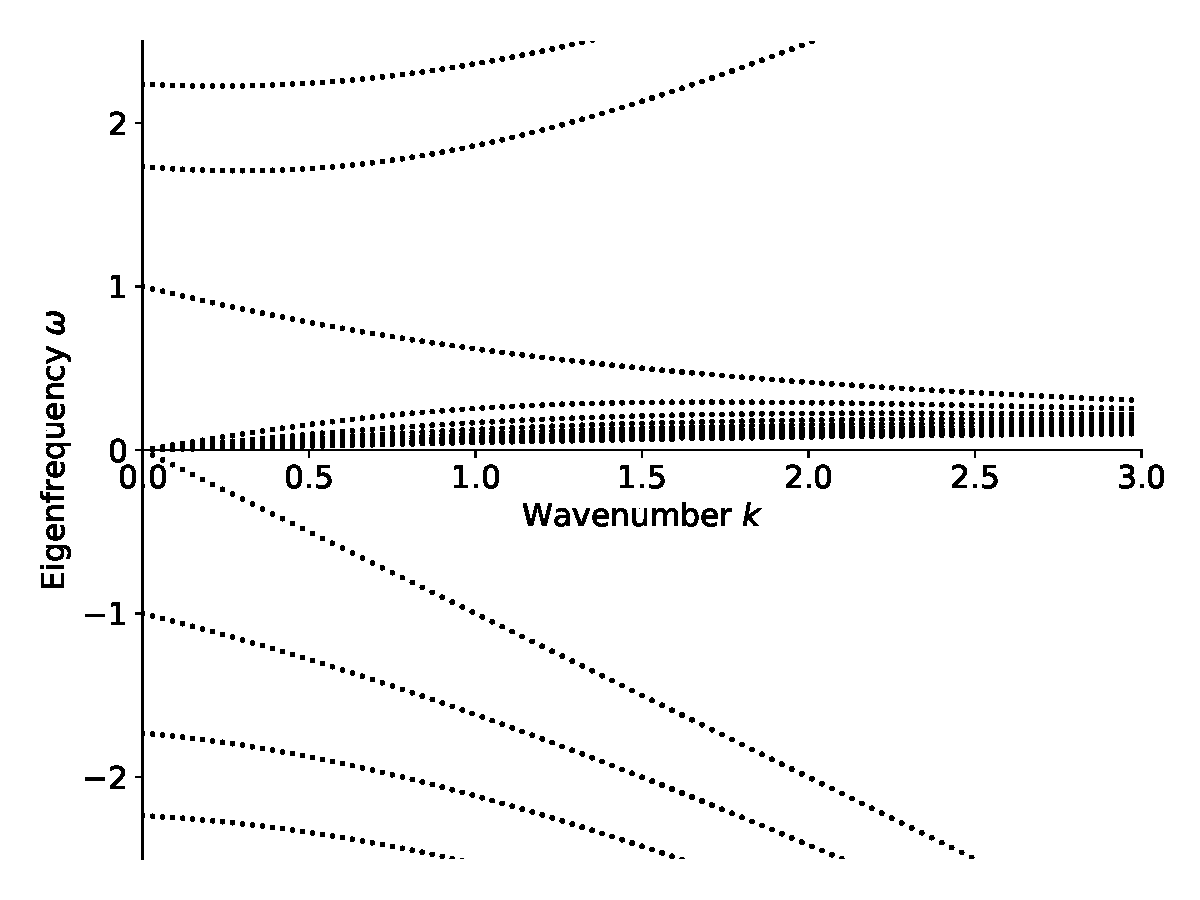
\includegraphics[width=0.7\textwidth]{figures/eqm-zonal-flow/disp-beta.pdf}
%   \caption{Dispersion relation on the beta-plane, calculated with spectral method giving the same results as the analytic solutions of \citet{matsuno1966quasi}.}
%   \label{fig:disp-beta}
% \end{figure}


The wave-1 forcing on a tidally locked planet is stationary and symmetric about the equator, so it will preferentially excite the lowest-order symmetric modes -- the Rossby and Kelvin modes. Figure \ref{fig:beta-plane-free-rossby} shows the free Rossby mode with zonal wavenumber 1. Its positive eigenvalue $\omega$ means that the free Rossby mode travels westwards (following the convention in \citet{matsuno1966quasi} for the relation between eigenvalue and direction of travel). Figure \ref{beta-plane-free-kelvin} shows the free Kelvin mode with zonal wavenumber 1. This is a special solution of the equations with zero meridional velocity, which has a negative eigenvalue so travels eastward as a free wave.

\begin{figure}
  \centering
  \begin{subfigure}[t]{0.49\textwidth}
    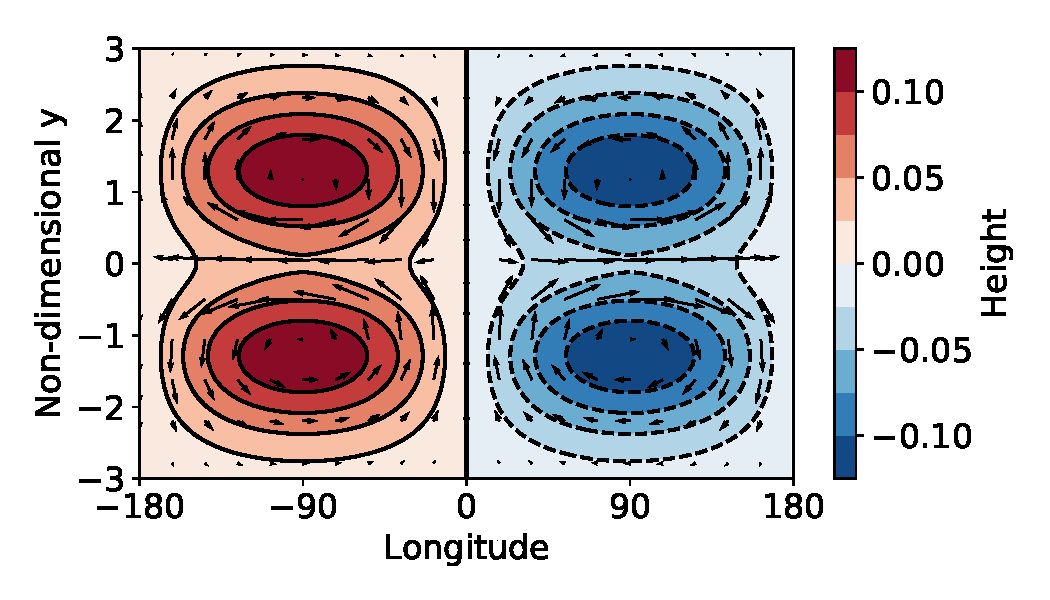
\includegraphics[width=1.0\textwidth]{figures/eqm-zonal-flow/beta-plane-free-rossby.pdf}
    \caption{Rossby wave.}
    \label{fig:beta-plane-free-rossby}
  \end{subfigure}
  %
  \begin{subfigure}[t]{0.49\textwidth}
    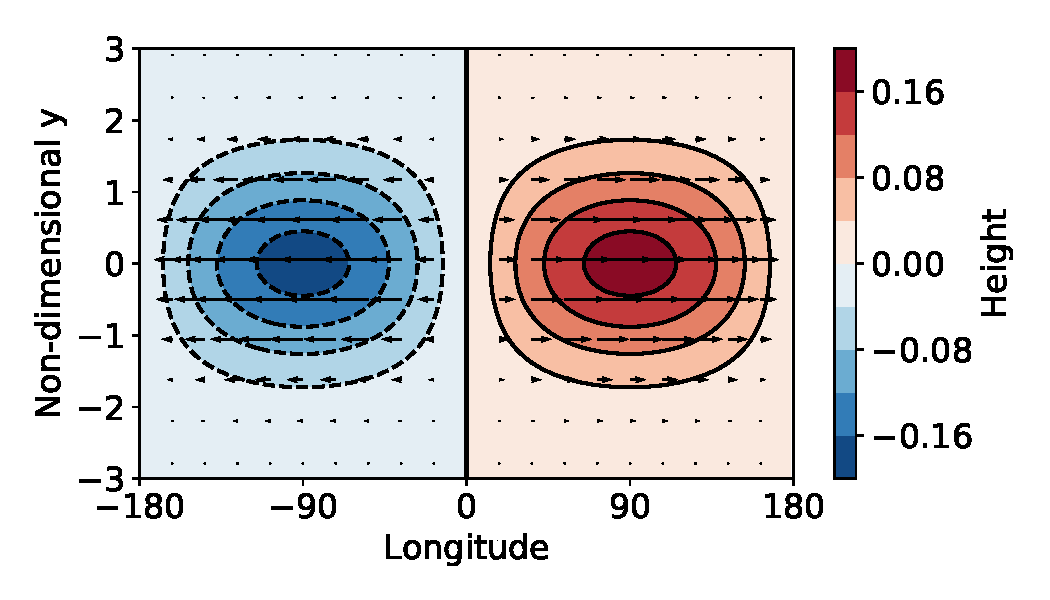
\includegraphics[width=1.0\textwidth]{figures/eqm-zonal-flow/beta-plane-free-kelvin.pdf}
    \caption{Kelvin wave.}
    \label{beta-plane-free-kelvin}
  \end{subfigure}
  \caption{The non-dimensional height and velocity fields of the lowest order free modes of a shallow-water system on an equatorial beta-plane. The response to forcing on a tidally locked planet is composed mainly of forced Rossby and Kelvin modes.}
  \label{fig:beta-plane-free-rossby-kelvin}
\end{figure}


%SUBSECTION -- RESPONSE TO FORCING
\subsection{Linear Response to Forcing}

\citet{showman2011superrotation} use this linear shallow-water model to represent the atmosphere of a tidally locked planet. A tidally locked planet is constantly heated on its day-side and cooled on its night-side, giving a stationary forcing very similar  to the forcing used in \citet{matsuno1966quasi}. This forcing $Q(x,y)$ acts on the $h$ field, giving the equations:

\begin{equation}\label{eqn:sw-eqns-forced}
  \begin{gathered}
    \alpha_{dyn} u - \beta y v +\frac{\partial h}{\partial x} = 0, \\
    \alpha_{dyn} v + \beta y u + \frac{\partial h}{\partial y} = 0, \\
    \alpha_{rad} h + c^{2}(\frac{\partial u}{\partial x} + \frac{\partial v}{\partial y}) = Q(x,y), \\
  \end{gathered}
\end{equation}

where both the dynamical and radiative damping rates $\alpha_{dyn}$ and $\alpha_{rad}$ are often set to a uniform damping $\alpha$ for a simpler solution. The boundary conditions are

\begin{equation}
  u , v , h \rightarrow 0 \quad \mathrm{for} \quad y \rightarrow \pm \infty.
\end{equation}

\citet{matsuno1966quasi} shows how the response of Equation \ref{eqn:sw-eqns-forced} to a forcing $Q(x,y) = Q_{0} \sin(x) e^{-y^{2}/2}$ and uniform damping $\alpha_{rad}=\alpha_{dyn}=\alpha$ can be found analytically as a sum of the free modes of the system.

The forced response $\chi = (u,v,h)$ is a sum of the free modes $\xi_{m}=(u_{m},v_{m},h_{m})$, weighted by coefficients $a_{m}$:

\begin{equation}
  \chi = \sum a _ { m } \xi _ { m },
\end{equation}

where the coefficients are

\begin{equation}
  a _ { m } = \frac { 1 } { \alpha - i \omega _ { m } } b _ { m },
\end{equation}

where $\omega_{m}$ is the eigenvalue of the mode $m$, and the projection of each mode onto the forcing is

\begin{equation}
  b _ { m } = \left[ \int \overline { \xi } _ { m } ( y ) \sigma ( y ) d y \right] / \left[ \int \left| \xi _ { m } ( y ) \right| ^ { 2 } d y \right].
\end{equation}

Figure \ref{fig:beta-plane-forced} shows the response to the forcing $Q(x,y) = Q_{0} \sin(x) e^{-y^{2}/2}$, where all the coefficients $a_{m}$ are zero apart from the Kelvin wave and $n=1$ Rossby wave. The Rossby wave appears west of the substellar point due to its positive eigenvalue $\omega_{m}$, and the Kelvin wave appears east of the substellar point due to its negative eigenvalue.

\begin{figure}
  \centering
  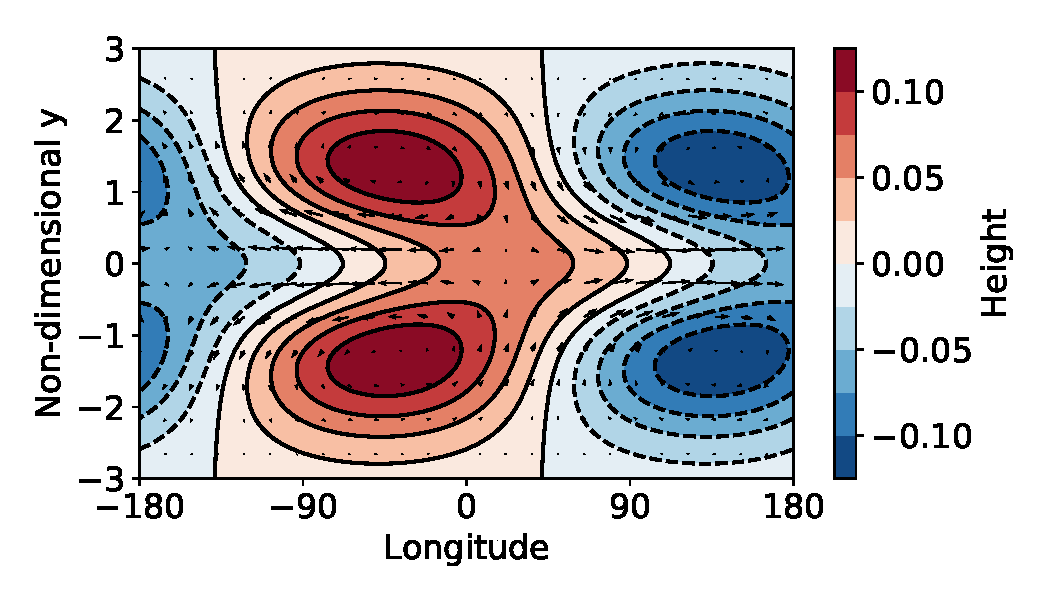
\includegraphics[width=0.65\textwidth]{figures/eqm-zonal-flow/beta-plane-forced.pdf}
  \caption{Non-dimensional response of Equation \ref{eqn:sw-eqns-forced} to forcing $Q(x,y) = Q_{0} \sin(x) e^{-y^{2}/2}$, showing the maximum of the Rossby wave west of the maximum of the forcing (the substellar point) and the maximum of the Kelvin wave east of this point.}\label{fig:beta-plane-forced}
\end{figure}


%SUBSECTION -- ACCELERATION
\subsection{Equatorial Acceleration}

The phase shift between the Rossby and Kelvin waves in the response to forcing produces an equatorward momentum transport that would be expected to produce equatorial superrotation \citep{showman2011superrotation, tsai2014three}. Zonally averaging the zonal momentum equation in Equation \ref{eqn:sw-eqns-1} gives the latitudinal acceleration profile \citep{thuburn1999zonalmean}:

\begin{equation}\label{eqn:zonal-mean-mom-no-R}
  \frac { \partial \overline { u } } { \partial t } = \underbrace { \overline { v } ^ { * } \left[ f - \frac { \partial \overline { u } } { \partial y } \right] } _ { I } \underbrace { - \frac { 1 } { \overline { h } } \frac { \partial } { \partial y } \left[ \overline { ( h v ) ^ { \prime } u ^ { \prime } } \right] } _ { I I } + \underbrace {  \frac { 1 } { \overline { h } } \overline { u ^ { \prime } Q ^ { \prime } } } _ { I I I } \underbrace { - \frac { \overline { u } ^ { * } } { \tau _ { \mathrm { drag } } } } _ { I V } - \frac { 1 } { \overline { h } } \frac { \partial \left( \overline { h ^ { \prime } u ^ { \prime } } \right) } { \partial t },
\end{equation}

where for a variable $X$, $\overline{X}^{*} = \overline{h X} / \overline{h}$. Figure \ref{fig:beta-fluxes-no-R} plots the terms in Equation \ref{eqn:zonal-mean-mom-no-R} for the response to forcing in Figure \ref{fig:beta-plane-forced}. It shows that the horizontal convergence of eastward momentum at the equator due to stationary eddies (term II) is exactly cancelled by the removal of eastward momentum from the equator by vertical momentum transport (term III). This means that the forced linear shallow-water model of \citet{matsuno1966quasi} does not accelerate at the equator, so a modification is needed to model the atmosphere of a tidally locked planet.

\begin{figure}
  \centering
  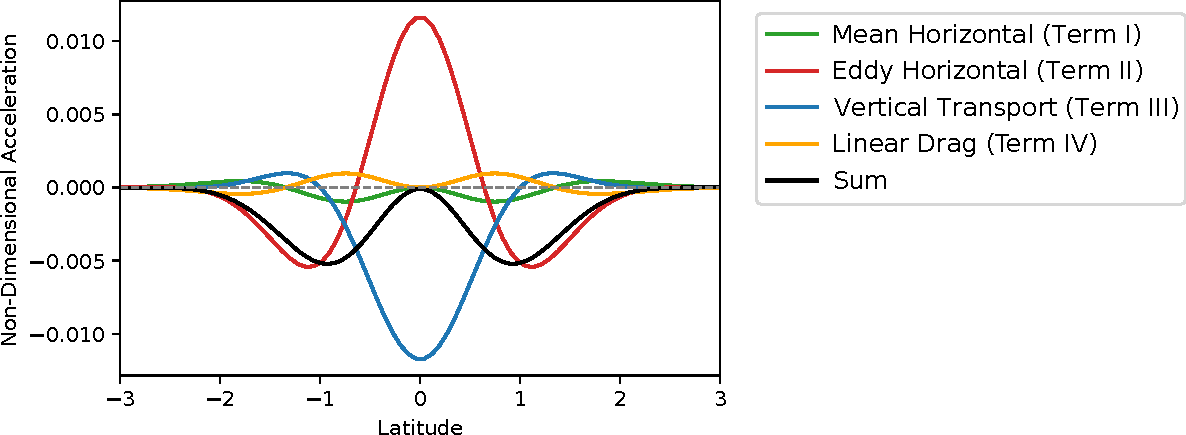
\includegraphics[width=1.0\textwidth]{figures/eqm-zonal-flow/beta-fluxes-no-R.pdf}
  \caption{Terms in the zonal-mean zonal momentum equation (Equation \ref{eqn:zonal-mean-mom-no-R}) without the correction $R$ to the momentum. The acceleration terms cancel exactly at the equator, which is why \citet{showman2010superrotation} introduced the correction $R$ to explain the formation of superrotation on tidally locked planets.}
  \label{fig:beta-fluxes-no-R}
\end{figure}

This can be explained by rewriting Equation \ref{eqn:zonal-mean-mom-no-R} in terms of the relative vorticity $\vec{\zeta}=\left(v_{x}-u_{y}\right) \hat{k}$ \citep{showman2011superrotation}:

\begin{equation}\label{eqn:zonal-mean-mom-zeta-no-R}
  \frac{\partial \overline{u}}{\partial t}=\overline{v^{\prime} \zeta^{\prime}}+\overline{v}(f+\overline{\zeta})-\frac{\overline{u}}{\tau_{\mathrm{drag}}},
\end{equation}

For forcing that is symmetric about the equator, the solutions are symmetric about the equator in $u$ and antisymmetric in $v$, so are also antisymmetric in $\zeta$. $v$ and $\zeta$ are therefore zero at the equator, so the first two terms in Equation \ref{eqn:zonal-mean-mom-zeta-no-R} are zero. This results in zero acceleration at the equator, for an atmosphere at rest with $\overline{u} = 0$.

\citet{showman2010superrotation} resolved this problem by introducing a correction $R$ to the mean vertical momentum transport. The correction represents the effect of advection between the active upper layer and quiescent lower layer \citep{shell2004superrotation}. \citet{showman2010superrotation} explain:

\textit{``Air moving out of the upper layer ($Q<0$) does not locally affect the upper layer’s specific angular momentum or wind speed, hence $R=0$ for that case. But air transported into the upper layer carries lower‐layer momentum with it and thus alters the local specific angular momentum and zonal wind in the upper layer.''}

Following \citet{shell2004superrotation}, they impose conservation of momentum between the stationary lower layer and the active upper layer, resulting in the correction:

\begin{equation}
  \mathbf{R}(\lambda, \phi, t)=\left\{\begin{array}{ll}{-\frac{Q \mathbf{v}}{h},} & {Q>0} \\ {0,} & {Q<0}\end{array}\right.
\end{equation}

\citet{shell2004superrotation} consider an axisymmetric planet where the air is rising at the equator and falling at the poles. In the tidally locked case, the air is rising at the substellar point and falling at the antistellar point. Figure \ref{fig:beta-plane-forced} shows that this term produces a net westerly acceleration at the equator. On the day-side where $Q>0$, the equatorial winds are mostly easterly, so $R$ is non-zero and positive, giving a westerly acceleration. On the night-side, $Q<0$ so there is no effect from $R$. This asymmetry in $R$ produces a net westerly acceleration at the equator.

Including the correction $R$, the zonal-mean momentum equation becomes:

\begin{equation}\label{eqn:zonal-mean-mom}
  \frac { \partial \overline { u } } { \partial t } = \underbrace { \overline { v } ^ { * } \left[ f - \frac { \partial \overline { u } } { \partial y } \right] } _ { I } \underbrace { - \frac { 1 } { \overline { h } } \frac { \partial } { \partial y } \left[ \overline { ( h v ) ^ { \prime } u ^ { \prime } } \right] } _ { I I } +\underbrace{\left[\frac{1}{\overline{h}} \overline{u^{\prime} Q^{\prime}}+\overline{R_{u}}^{*}\right]}_{\text { III }} \underbrace { - \frac { \overline { u } ^ { * } } { \tau _ { \mathrm { drag } } } } _ { I V } - \frac { 1 } { \overline { h } } \frac { \partial \left( \overline { h ^ { \prime } u ^ { \prime } } \right) } { \partial t },
\end{equation}

and in vorticity form, it is:

\begin{equation}\label{eqn:zonal-mean-mom-zeta-no-R}
\frac{\partial \overline{u}}{\partial t}=\overline{v^{\prime} \zeta^{\prime}}+\overline{v}(f+\overline{\zeta})-\frac{\overline{u}}{\tau_{\mathrm{drag}}}+\overline{R_{u}}.
\end{equation}

\begin{figure}[t]
  \centering
  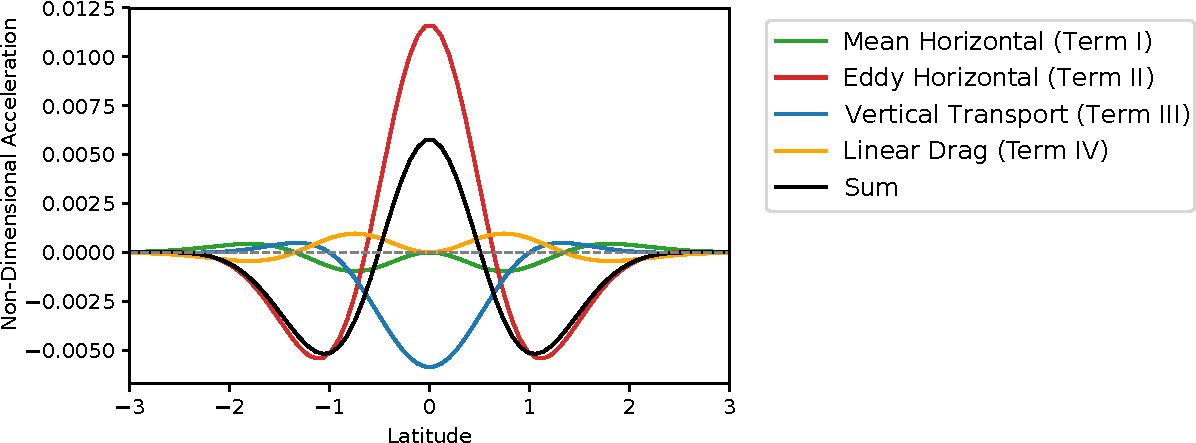
\includegraphics[width=1.0\textwidth]{figures/eqm-zonal-flow/beta-fluxes.pdf}
  \caption{Terms in the zonal-mean zonal momentum equation (Equation \ref{eqn:zonal-mean-mom}) with the correction $R$ to the momentum. The correction reduces the ``Vertical Transport'' term in Figure \ref{fig:beta-fluxes-no-R}, giving a net eastward acceleration at the equator.}
  \label{fig:beta-fluxes-with-R}
\end{figure}

Therefore, there is a positive acceleration on the equator unlike in Equation \ref{eqn:zonal-mean-mom-zeta-no-R}. Figure \ref{fig:beta-fluxes-with-R} shows the net positive acceleration at the equator due to the reduced ``Vertical Transport'' term (Term III in Equation \ref{eqn:zonal-mean-mom}). This explains the formation of eastward equatorial flow in the atmospheres of tidally locked planets. However, Figure \ref{fig:beta-fluxes-with-R} shows that this eastward equatorial flow requires westward flow at high latitudes, which is inconsistent with some GCM simulations. The next section will introduce the GRW mechanism to resolve this problem.



%
% %SUBSECTION -- SR and SBR
% \subsection{Super- and Sub-Rotation}\label{sec:super-sub-rotation}
%
% It is important to define the concept of ``superrotation'' precisely, to make the proposed effect of the meridional circulation clear. \citet{read2018superrotation} defines superrotation using the ``superrotation index'', which is a relative angular momentum excess compared to solid-body rotation at the equator \citep{read1986super}. The specific angular momentum $m$ is:
%
% \begin{equation}
%   m=a \cos \phi(\Omega a \cos \phi+u),
% \end{equation}
%
% and the local superrotation index is:
%
% \begin{equation}
%   s=\frac{m}{\Omega a^{2}}-1
% \end{equation}
%
% This provides a measure of the local momentum excess provided by momentum fluxes in the atmosphere -- generally, equatorward fluxes which produce a positive superrotation index. The global superrotation index is a mass-weighted integral of the local quantity:
%
% \begin{equation}
%   S_{m}=\frac{\iiint \rho m \mathrm{d} V}{\iiint \rho \Omega a^{2} \cos ^{2} \phi \mathrm{d} V}-1.
% \end{equation}
%
% \citet{read2018superrotation} highlights that $s$ and $S_{m}$ cannot exceed zero without up-gradient fluxes of angular momentum, a condition referred to as Hide's Theorem \citep{hide1969dynamics}. On a tidally locked planet, these are provided by the stationary horizontal eddy momentum fluxes discussed previously and shown in Figure \ref{fig:beta-fluxes-with-R}.
%
% The distinction between superrotating and subrotating flow, versus westerly and easterly flow, is vital to the conclusions of this chapter. The fluxes shown in Figure \ref{fig:beta-fluxes-with-R} operates on a background flow of zero. Therefore, any westerly flow at the equator requires easterly flow at high latitudes to conserve angular momentum. The GRW mechanism used in this chapter applies this system to a non-zero background flow, with a meridional circulation and westerly subtropical jet. Then, the equatorward momentum transport produces westerly superrotating flow at the equator -- but, it does not necessarily need to be compensated by easterly flow as before. Instead, it must be compensated by more subrotating flow (lower $s$) at higher latitudes. This subrotating flow can still be westerly, leading to the westerly flow at all latitudes seen in some GCM simulations.


%%%%%%%%%%%%%%%%%%%%%%%%%%%%
%SECTION 2 -- MERIDIONAL CIRCULATION
\section{Linear Model of the GRW Mechanism}

The meridional circulation of an atmosphere is driven by a difference in forcing between its equator and pole. On the Earth, it consists of multiple overturning cells that are approximately zonally uniform. The instellation on tidally locked planets is not zonally uniform so the meridional circulation should vary with longitude. Some studies have measured aspects of the meridional circulation of tidally locked planets in simulations of hot Jupiters and sub-Neptunes \citep{charnay20153d, showman2015circulation, mendoncca2018revisiting}. These studies did not consider the effect of the meridional circulation on the zonal flow, which I will discuss here.

The previous section showed that the linear shallow-water model of \citet{showman2010superrotation} explains the formation of equatorial superrotation, but requires westward flow at high latitudes to conserve angular momentum. This is not consistent with many GCM simulations that have eastward flow at all latitudes at the level of their equatorial jet \citep{kataria2015atmospheric,showman2015circulation,pierrehumbert2018review}. The shallow-water model is also not consistent with the evolution of angular momentum seen in GCM simulations. It predicts that the jet layer must lose angular momentum, as the only exchange of momentum out of the layer is a net loss to the lower layer via term III in Equation \ref{eqn:zonal-mean-mom}. Many simulations of tidally locked planets have positive net angular momentum at the level of their jet (and in total in their atmosphere) so contradict the linear model \citep{heng2015review, pierrehumbert2018review}.

Both of these problems could be resolved by a process that adds eastward acceleration to the jet layer at high latitudes. This section will suggest that the meridional circulation is this process, forming eastward subtropical jets via the ``Gierasch-Rossow-Williams'' mechanism that also produces the equatorial jet. I will demonstrate this mechanism in a linear and non-linear shallow-water models and an idealised GCM.


% This section will show how the predicted zonal flow in the linear shallow-water model of \citet{showman2011superrotation} can be inconsistent with GCM simulations. It will then introduce the GRW mechanism to resolve this problem, and modify the linear model to represent the effect of this mechanism. The following sections will demonstrate the mechanism in a non-linear shallow-water model and an idealised GCM.


% In this section, I will show that the linear shallow-water model of \citet{showman2011superrotation} is not consistent with some aspects of the zonal flow produced in GCM simulations of tidally locked planets. The shallow-water model requires easterly flow at high latitudes if there is to be westerly equatorial superrotation, but some GCM simulations have westerly flow at all latitudes at the level of their jet.

% I will introduce the Gierasch-Rossow-Williams (GRW) mechanism as a way to reconcile these differences. This mechanism combines the momentum transport of a meridional circulation with the equatorward momentum transport of the \citet{showman2011superrotation} mechanism (it was originally used to explain the superrotation of the atmosphere of Venus). I will show that the zonal mean meridional circulation can be considered to only depend on the zonal mean of the forcing, avoiding the difficult question of its longitudinal variation.
%
% The GRW mechanism then allows for westerly flow at all latitudes, as it pumps westerly momentum into the atmosphere from the surface and transports it to high latitudes. I will demonstrate this mechanism at work in a linear shallow-water model, a non-linear shallow-water model, and the GCM Exo-FMS. I will show that it requires subrotating (not superrotating) flow at high latitudes -- but this subrotating flow can still be westerly.


% %SUBSECTION -- PROBLEM WITH ACCELERATION AND MOMENTUM
% \subsection{Angular Momentum in the Shallow-Water Model}



%SUBSECTION -- PROPOSED MECHANISM
\subsection{The GRW Mechanism on a Tidally Locked Planet}\label{sec:grw-on-tl}

% In this section, I will introduce the GRW mechanism and show how it can be applied to a tidally locked planet. I will demonstrate that the zonal-mean meridional circulation -- a vital part of the mechanism -- can be approximated as only due to the zonal mean of the forcing, avoiding the complicated longitudinal variation of the meridional circulation.

The ``Gierasch-Rossow-Williams'' (GRW) mechanism was developed by \citet{gierasch1975meridional} and \citet{rossow1979large} to describe the formation of zonal flow in the atmosphere of Venus \citep{read2018superrotation}. Figure \ref{fig:gierasch} shows the GRW mechanism with the momentum fluxes particular to a tidally locked planet.
%
% In the mechanism, a mean meridional circulation has a westerly drag applied to the easterly flow in its lower branch. The westerly angular momentum added to the lower branch is then conveyed to the whole atmosphere by the meridional circulation. This circulation produces ``subtropical'' jets at high latitudes to conserve angular momentum as the upper branch travels towards the poles

The solid arrows in Figure \ref{fig:gierasch} show the momentum transport of the mean meridional circulation. I will explain later why this is treated as a zonal-mean process when it varies with longitude in reality. Hot air rises at the equator and travels towards the poles, accelerating eastward to conserve angular momentum. It falls at the poles, and then returns to the equator, accelerating westward to conserve momentum again. Drag from the surface applies a westerly torque to this lower branch, adding prograde eastward momentum to the entire atmosphere. The net effect of this mean meridional circulation is to produce eastward subtropical jets at high latitudes, and a total positive eastward atmospheric angular momentum. The ideal mechanism applies to a planet with a global Hadley cell, avoiding the multiple cells and jets seen on Earth.

The dashed lines in Figure \ref{fig:gierasch} show the momentum transport due to the wavenumber-1 ``eddy'' stationary wave response to day-night forcing \citep{showman2011superrotation}. The horizontal momentum flux in Figure \ref{fig:beta-fluxes-with-R} transports angular momentum towards the equator. This produces the eastward equatorial jet and applies a westward acceleration at high latitudes, which is opposed by the eastward acceleration at high latitudes due to the meridional circulation. I will show later that the horizontal and vertical transports balance at the equator in equilibrium, and the horizontal eddy transport balances the mean meridional transport at high latitudes.

This mechanism can resolve the problems introduced at the start of this section. The atmosphere and jet layer gain positive net angular momentum from the drag on the lower branch of the mean meridional circulation. The jet layer can have eastward flow at all latitudes, as the due to the westward acceleration at high latitudes in Figure \ref{fig:beta-fluxes-with-R} is opposed by the eastward acceleration from the meridional circulation. Instead of requiring westward flow at high latitudes to balance the eastward flow at the equator, this mechanism requires subrotating flow at high latitudes to balance the superrotating flow at the equator -- but, the subrotating flow can still be eastward.

\begin{figure}
  \centering
  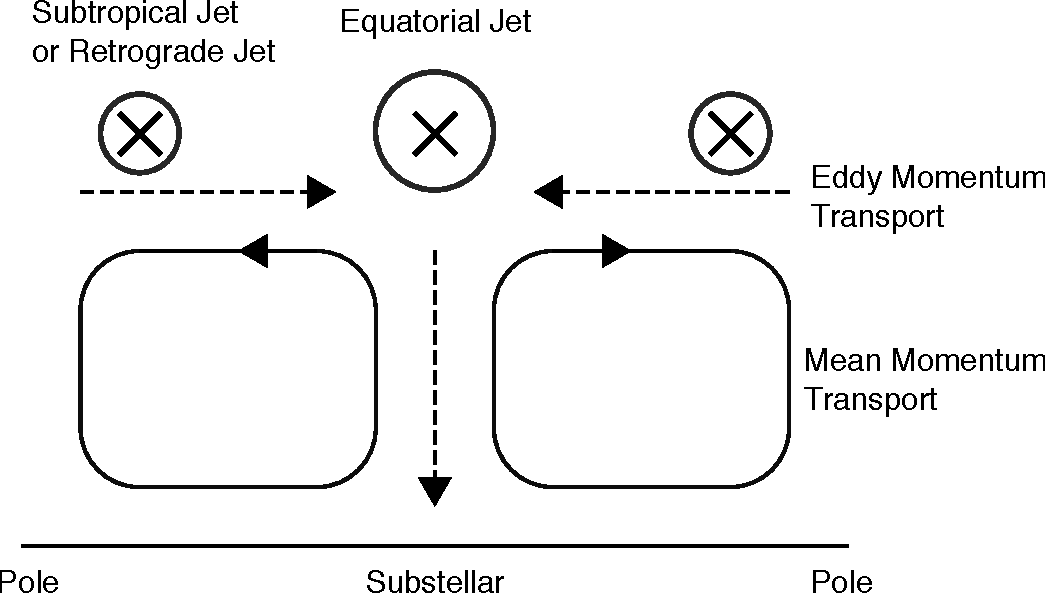
\includegraphics[width=0.75\textwidth]{figures/eqm-zonal-flow/gierasch-tl.pdf}
  \caption{The Gierasch-Rossow-Williams (GRW) mechanism \citep{read2018superrotation}, applied to the atmosphere of a tidally locked terrestrial planet. The solid line shows the mean momentum transport, which produces subtropical jets at high latitudes. The dashed lines show the horizontal and vertical momentum transports, which accelerate and decelerate the equatorial superrotation respectively.}
  \label{fig:gierasch}
\end{figure}


%%%%%%



% Figure \ref{fig:gierasch} shows the GRW mechanism \citep{read2018superrotation} as applied to the atmosphere of a tidally locked planet. The solid lines show the mean meridional circulation, which transports air up from the equator and poleward in the jet layer. It accelerates in this upper branch to conserve angular momentum as it travels poleward, creating westerly subtropical jets. The equatorward lower branch accelerates westward for the same reason and is dragged by the surface. This produces a net eastward torque on the atmosphere, which is conveyed to the upper layer by the meridional circulation. This results in a net positive angular momentum in both the jet layer and in the whole atmosphere.

% The dashed lines show the momentum transport terms due to the stationary wave response in a tidally locked planet \citep{showman2011superrotation}. These transport angular momentum equatorward in the jet layer, and downward at the equator. Later, I will show how they balance each other at the equator, and the transport from the mean meridional circulation at higher latitudes. This will explain how the number of zonal jets and their relative strength depends on the planetary parameters.

The idealised GRW mechanism in Figure \ref{fig:gierasch} assumes that the meridional circulation has the same zonal-mean effect on a tidally locked planet as on an asynchronously rotating planet like Venus. This ignores the longitudinal variation in this circulation due to the longitudinal variation in the equator-pole temperature gradient. In reality, the meridional circulation will be strongest at the substellar longitude, and negligible or even reversed on the night-side \citep{charnay20153d}. However, I will show that in the linear limit only the zonal mean of the meridional circulation is relevant to the momentum transport and jet formation discussed above.


%
% This provides an idealised picture of the momentum transports that produce the zonal flow on a tidally locked planet. However, it only applies to the zonal mean flow, and the zonal mean of the meridional circulation. In reality, the meridional circulation on a tidally locked planet will vary greatly with longitude. \citet{charnay20153d} suggests an ``anti-Hadley'' circulation of cells in the opposite direction to Hadley cells on the night-side of a tidally locked planet.
%
% This may make it difficult to apply the GRW mechanism in this case, as it relies on the zonal mean of the meridional circulation. However, I will show here that in the linear limit the meridional circulation on a tidally locked planet has a zonal mean that only depends on the zonal mean of the instellation -- so, the details of its longitudinal variation do not matter to the mechanism.
%
% LINEAR LIMIT INTRO
%
% Now, I will show that in the linear limit the meridional circulation is only governed by the zonal mean of the forcing (the zeroth-order term in Figure \ref{fig:decomp-forcing}).

\citet{held1980nonlinear} show that the properties of the meridional circulation 0-- zonal and meridional velocities, meridional momentum flux etc. -- are linear with response to the forcing. This holds separately at every longitude. The linearity of any property $X$ with respect to the forcing $Q(\phi,\lambda)$ means that for axisymmetric forcing, the zonal mean of $X$ has the property:

\begin{equation}
  \overline{X} \sim \overline{Q} =Q_{0}\cos{\phi}.
\end{equation}

For the same forcing on a tidally locked planet, the forcing is $ Q(\phi,\lambda)=Q_{0}\cos{\phi}\sin{\lambda}$ on the day-side, plus a uniform relaxation on the night-side. So, the zonal mean is:

\begin{equation}
  \overline{X} \sim \overline{Q} =Q_{0}\cos{\phi}\overline{\sin\lambda},
\end{equation}

where the mean of the $\sin \lambda$ is only taken over the day-side, giving:

\begin{equation}
  \overline{X} \sim Q_{0}\cos{\phi},
\end{equation}

The zonal mean of the meridional circulation therefore depends on the zonal mean of the forcing, when the local meridional circulation depends linearly on the local forcing. It is therefore possible to consider the zonal-mean effect of the meridional circulation on a tidally locked planet as entirely due to the wave-0 (zonal mean) component of the forcing. It is possible that non-linear effects from high forcing magnitudes or interactions with the zonal flow will make this assumption invalid.

% The accuracy of this approximation will be tested by how well it describes the results of GCM simulations later in this chapter.



%SUBSECTION -- LINEAR
\subsection{Demonstration in a Linear Shallow-Water Model}\label{sec:lin-sw-grw-results}

This section demonstrates the GRW mechanism on a tidally locked planet in a modified version of the linear shallow-water model of \citet{showman2011superrotation}. The model is modified by adding a zonally uniform meridional velocity $\overline{V}(y) = V_{0} \sin{y/y_{0}} e^{-y^{2}/y_{0}^{2}}$ to represent the poleward branches of the meridional circulation. The meridional scale is $y_{0}=\sqrt{2}$ as before and in \citet{matsuno1966quasi}, and the scale of the velocity is $V_{0} = 0.02$, chosen to produce an appropriate acceleration magnitude for this demonstration.


% Figure \ref{fig:beta-fluxes-plus-merid} shows the zonal-mean zonal acceleration in this linear model, when a zonally uniform background meridional velocity $\overline{V}(y) = V_{0} \sin{y/y_{0}} e^{-y^{2}/2}$ is imposed.



\begin{figure}
  \centering
  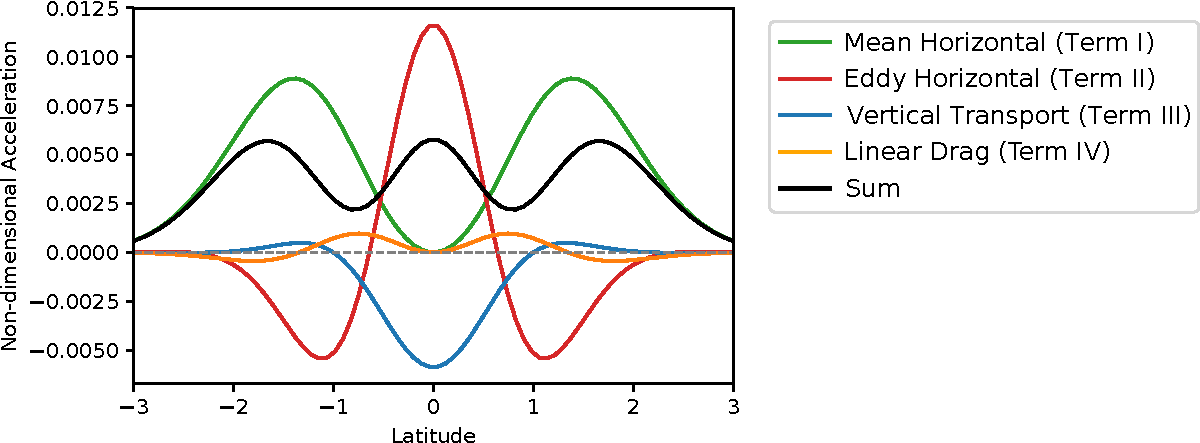
\includegraphics[width=1.0\textwidth]{figures/eqm-zonal-flow/beta-fluxes-plus-merid.pdf}
  \caption{Acceleration terms in the zonal-mean zonal momentum equation (Equation \ref{eqn:zonal-mean-mom}), with an imposed uniform zonal-mean meridional velocity $\overline{V}(y) = V_{0} \sin{y/y_{0}} e^{-y^{2}/y_{0}^{2}}$, showing prograde westerly acceleration at all latitudes.}
  \label{fig:beta-fluxes-plus-merid}
\end{figure}

% Figure \ref{fig:beta-fluxes-with-R} showed how the linear shallow-water model in \citet{showman2011superrotation} predicts equatorial superrotation, but requires easterly acceleration at high latitudes. In this chapter, I have intoduced the idea that a meridional circulation can produce westerly acceleration at high latitudes, resulting in westerly flow at all latitudes. This can be demonstrated simply in a modified version of the linear shallow-water model.

The imposed meridional velocity affects Term I in Equation \ref{eqn:zonal-mean-mom}, producing a westerly acceleration at high latitudes around the peak of the imposed meridional flow $\overline{V}(y)$. This opposes the easterly acceleration due to horizontal momentum transport from stationary eddies in the previous linear model, producing westerly prograde acceleration at all latitudes if the meridional velocity is large enough. In the GRW mechanism, this reflects the fact that the equatorward momentum transport from stationary eddies is moving momentum from a region that is already accelerated eastward by the meridional circulation.

So, rather than requiring easterly flow above a certain latitude as in the linear model of \citet{showman2011superrotation}, this model requires sub-rotating flow above a certain latitude -- but, the flow can still be eastward. Next, I will use a non-linear shallow-water model and a GCM to demonstrate the mechanism without needing to impose the meridional circulation, as it will emerge naturally from the forcing in the models.

 % An additional problem is that the forcing in the idealised linear shallow-water model of \citet{showman2011superrotation} has zero zonal mean, which suggests that there is no meridional circulation at all.



%%%%%%%%%%%%%%%%%%%%%%%%%%%%
%SECTION 3 -- NONLINEAR MODEL
\section{Non-Linear Model of the GRW Mechanism}\label{sec:nonlin-shallow}

This section demonstrates the GRW mechanism in a non-linear time-stepped shallow-water model. The meridional circulation and the acceleration at high latitudes will emerge naturally from the forcing field, unlike in the linear model where the meridional velocity was imposed. I will show that the equilibrium zonal flow is governed by the balance of momentum fluxes predicted by the GRW mechanism.



%%%%%%


 %I will show the effect of the realistic radiative-equilbrium forcing field introduced earlier, and the effects of its wave-0 and wave-1 forcing components.

  % The balance of momentum fluxes for steady-state zonal flow is the same in this non-linear model as in the GCM and in the linear shallow-water model, suggesting that the GRW mechanism is a robust description of the formation of this zonal flow.

%SUBSECTION --
\subsection{Non-Linear Shallow-Water Model}

The GFDL Spectral Dynamical Core\footnote{\url{gfdl.noaa.gov/idealized-spectral-models-quickstart/}} solves the equations describing the fluid dynamics of a model atmosphere by representing the solution as a series of spherical harmonic functions \citep{polvani2004numerically}. In this section, it is configured to solve the non-linear shallow-water equations in a single layer \citep{showman2011superrotation}. The non-linear shallow-water equations in this model\footnote{\url{gfdl.noaa.gov/wp-content/uploads/files/user_files/pjp/shallow.pdf}} retain the terms that are discarded by the linear shallow-water equations in the previous section. The model is forced by relaxation to a radiative equilibrium height field $h_{eq}$, where a tendency $\Delta h$ is applied to the height field $h$ at every timestep:

\begin{equation}
  \Delta h = \Delta t (h - h_{eq}) / \tau_{rad} ,
\end{equation}

where $\Delta t$ is the timestep and $\tau_{rad}$ is the thermal damping timescale. The only other forcing is the correction $R$ to the zonal momentum \citep{shell2004superrotation}. The model could apply dynamical damping to the velocity fields of the shallow-water layer, but I chose not to use this damping in order to match the GCM simulations better. Section \ref{sec:gcm-sim-grw} will show that dynamical damping is not part of the balance of forces on the jet in the GCM.

I ran three simulations in the model which were forced by relaxation to different radiative equilibrium height fields $h_{eq}$. The models were run for 100 days, and the results taken over the last 10 days after a steady state had formed.  All the tests in this section have $h_{0} = \SI{10}{\kilo\metre}$, $\Delta h = \SI{1}{\kilo\metre}$, and a thermal damping time $\tau_{rad}=$ 0.1 days. Figures \ref{fig:nonlin-test-A}, \ref{fig:nonlin-test-B}, and \ref{fig:nonlin-test-C} show the height fields and zonal-mean zonal and meridional velocities of each test.




% he non-zero wave-0 component shows that there is a non-zero zonal-mean forcing on the atmosphere which will produce a mean meridional circulation. The wave-1 component is the forcing considered by \citet{showman2011superrotation}, which produces the equatorial superrotation.

%TODO: WAVE 1 AND 0 COMPONENTS HAVE SIMILAR OR SAME MAGNITUDE



%SUBSECTION --
\subsection{Test A: Sinusoidal Forcing}



\begin{figure}
  \centering
  \begin{subfigure}[t]{0.52\textwidth}
    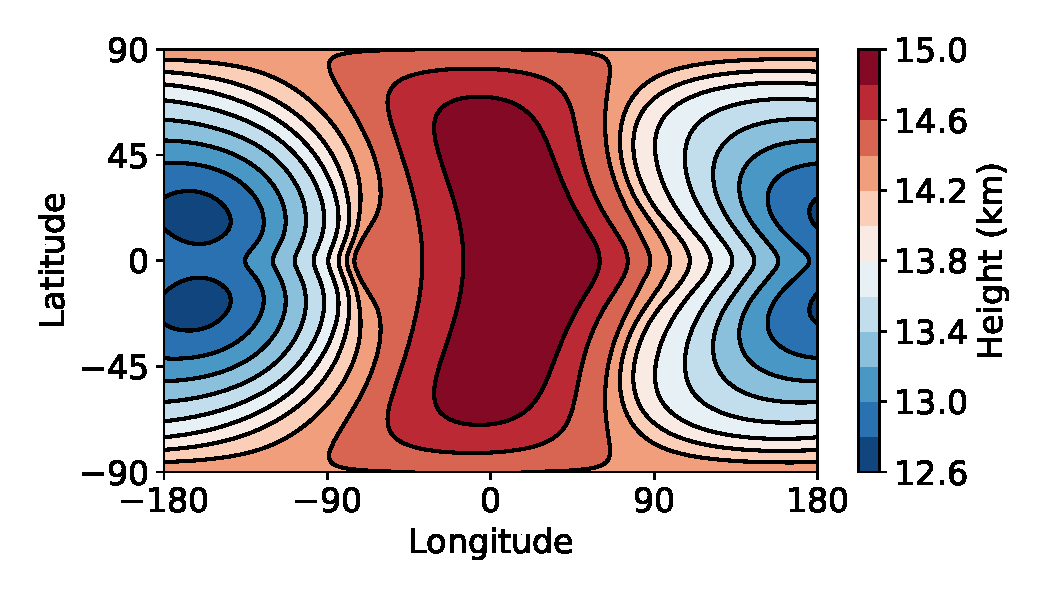
\includegraphics[width=1.0\textwidth]{figures/eqm-zonal-flow/test-A-h.pdf}
    \caption{Equilibrium height field.}
    \label{fig:test-A-h}
  \end{subfigure}
  %
  \begin{subfigure}[t]{0.47\textwidth}
    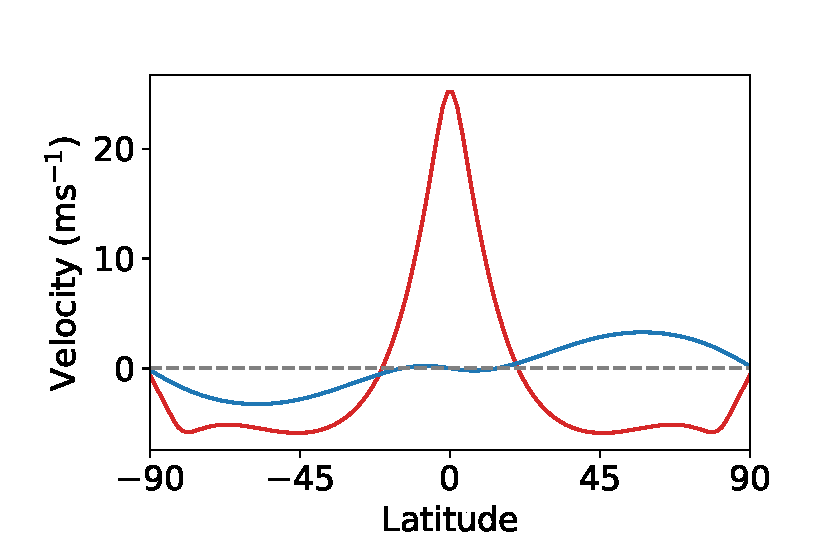
\includegraphics[width=1.0\textwidth]{figures/eqm-zonal-flow/test-A-u-v.pdf}
    \caption{$\overline{U}(y)$ (red) and $\overline{V}(y)$ (blue).}
    \label{fig:test-A-u-v}
  \end{subfigure}
  \caption{Test A with sinusoidal day-night forcing, showing the equilibrium height field, the zonal-mean zonal velocity $\overline{U}(y)$ (red), and the zonal-mean meridional velocity $\overline{V}(y)$ (blue). The height field shows the stationary wave response that produces an eastward equatorial jet and westward flow at high latitudes.}
  \label{fig:nonlin-test-A}

  \centering
  \begin{subfigure}[t]{0.52\textwidth}
    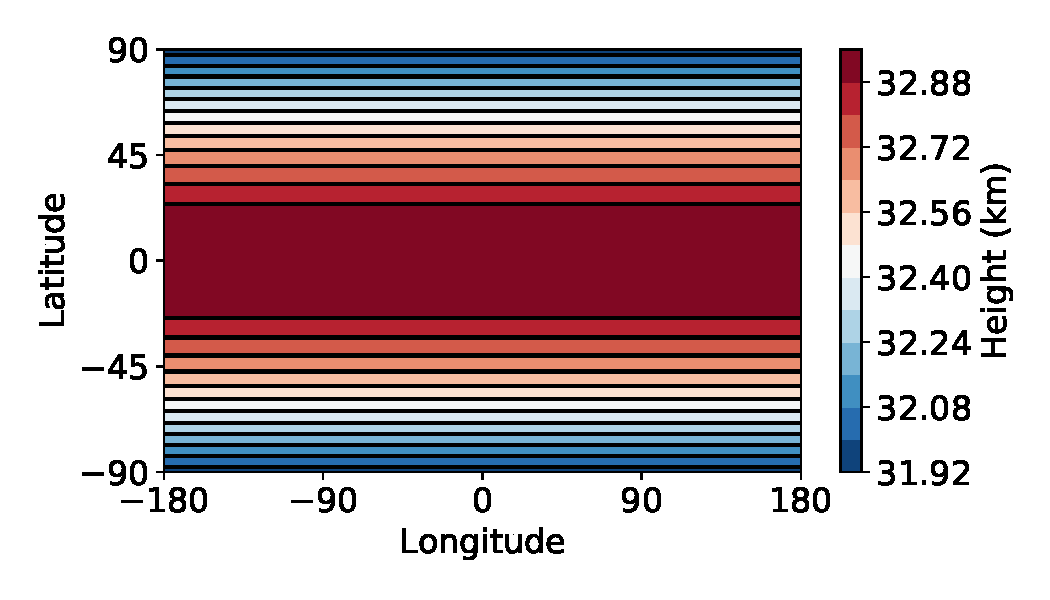
\includegraphics[width=1.0\textwidth]{figures/eqm-zonal-flow/test-B-h.pdf}
    \caption{Equilibrium height field.}
    \label{fig:test-B-h}
  \end{subfigure}
  %
  \begin{subfigure}[t]{0.47\textwidth}
    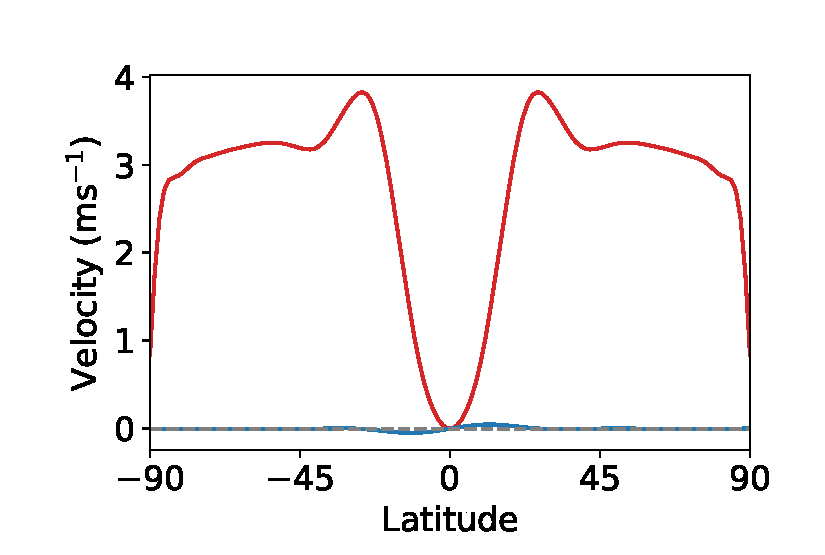
\includegraphics[width=1.0\textwidth]{figures/eqm-zonal-flow/test-B-u-v.pdf}
    \caption{$\overline{U}(y)$ (red) and $\overline{V}(y)$ (blue).}
    \label{fig:test-B-u-v}
  \end{subfigure}
  \caption{Test B with axisymmetric forcing, showing the axisymmetric height field and the meridional velocity that produces eastward subtropical jets.}
  \label{fig:nonlin-test-B}

  \centering
  \begin{subfigure}[t]{0.52\textwidth}
    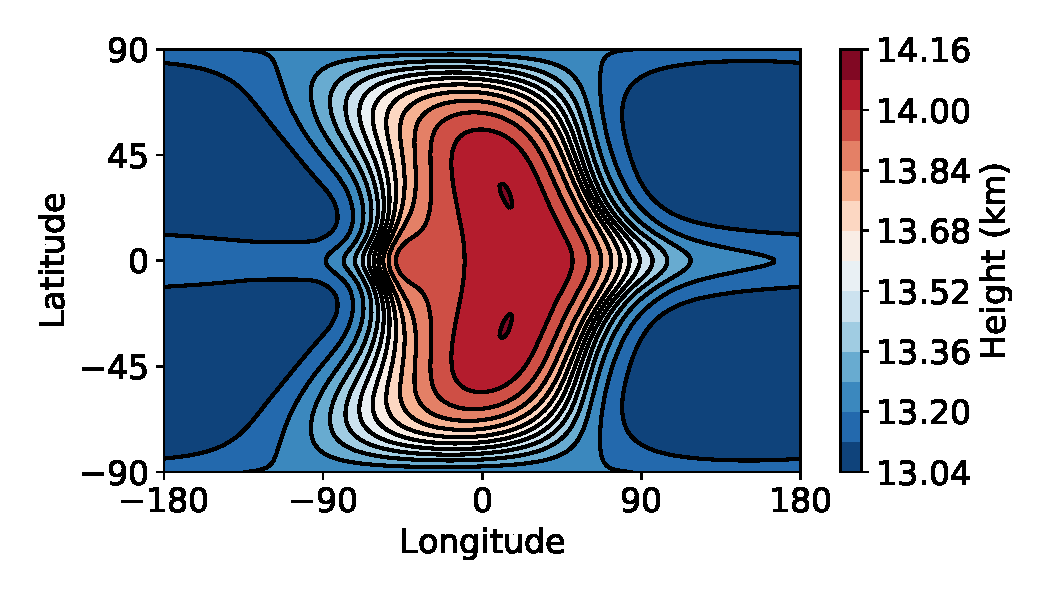
\includegraphics[width=1.0\textwidth]{figures/eqm-zonal-flow/test-C-h.pdf}
    \caption{Equilibrium height field.}
    \label{fig:test-C-h}
  \end{subfigure}
  %
  \begin{subfigure}[t]{0.47\textwidth}
    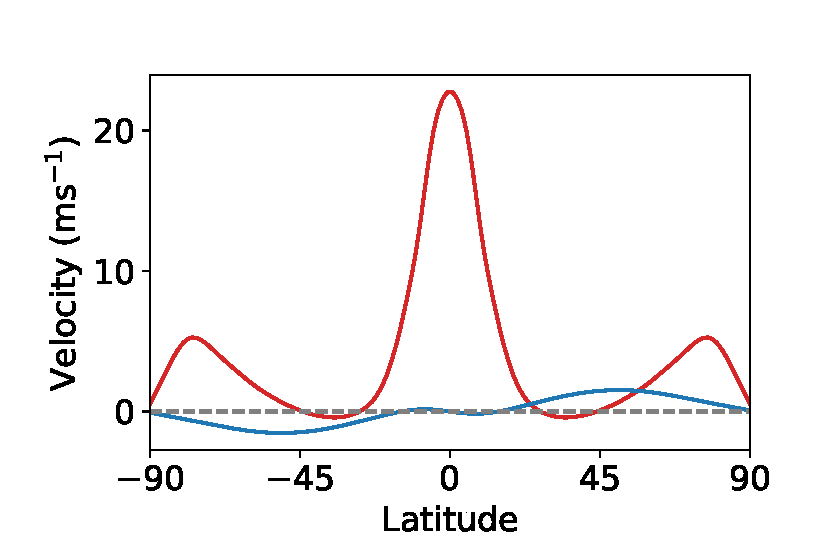
\includegraphics[width=1.0\textwidth]{figures/eqm-zonal-flow/test-C-u-v.pdf}
    \caption{$\overline{U}(y)$ (red) and $\overline{V}(y)$ (blue).}
    \label{fig:test-C-u-v}
  \end{subfigure}
  \caption{Test C with realistic forcing, showing the stationary wave response and the meridional velocity, which together produce eastward flow at all latitudes by the GRW mechanism.}
  \label{fig:nonlin-test-C}
\end{figure}


Test A was forced by relaxation to a radiative-equilibrium height field that varies sinusoidally with longitude:

\begin{equation}
  h_{eq} = h_{0} + \Delta h \sin \lambda \cos\phi.
\end{equation}

This is the same as the forcing field used in the linear model of \citet{matsuno1966quasi} and the non-linear model of \citet{showman2011superrotation}. It is a simple representation of day-side heating and night-side cooling, but does not produce a mean meridional circulation as it has zero zonal mean.

Figure \ref{fig:test-A-h} shows the resulting height field in equilibrium, which is similar to the non-linear simulations in Figure 8 of \citet{showman2011superrotation}. The model is forced in the same way as the linear response in Figure \ref{fig:beta-plane-forced}, but the non-linearity produces a day-night asymmetry in this case. The stationary waves created by the forcing transport eastward momentum towards the equator, producing an eastward equatorial jet and westward flow at high latitudes shown in Figure \ref{fig:test-A-u-v}. Note that there is some meridional velocity due to the small day-night asymmetry from the non-linear terms, but it is not strong enough to produce eastward subtropical jets. The stationary waves are partly shifted eastwards by this zonal-mean zonal velocity. As shown in Section \ref{sec:lin-sw-model}, the sinusoidal forcing must produce westward flow at high latitudes to balance the eastward flow at the equator, so is inconsistent with GCM simulations that can have eastward flow at all latitudes at the level of the jet \citep{showman2015circulation,kataria2015atmospheric,pierrehumbert2018review}.


%SUBSECTION --
\subsection{Test B: Axisymmetric Forcing}

The GRW mechanism requires a meridional circulation that produces eastward flow at the level of the jet at high latitudes. \citet{shell2004superrotation} model the meridional circulation of the Earth in a non-linear shallow-water model with an axisymmetric forcing with an equator-pole gradient. This produces a meridional velocity and eastward subtropical jets. The single-layer model does not represent the lower branch of the circulation, which would produce westward zonal flow. This will be represented in the GCM simulations later, where the westward surface flow will be a source of eastward atmosphere angular momentum due to Rayleigh drag.

Test B uses a simplified axisymmetric field to qualitatively reproduce the Earth-like circulation in \citet{shell2004superrotation}, and to show that a forcing field with a non-zero zonal mean produces an acceleration at high latitudes. The axisymmetric field is:

\begin{equation}
  h_{eq} = h_{0} + \Delta h \cos\phi / \pi.
\end{equation}

Figure \ref{fig:test-B-h} shows the axisymmetric height field in equilibrium, with a small equator-pole height gradient due to the forcing. The height gradient produces the meridional velocity shown in Figure \ref{fig:test-B-u-v}, that results in eastward zonal subtropical jets. Note that there is zero zonal flow at the equator. The next test will show how these subtropical jets are modified by equatorward momentum transport from the stationary wave forcing in Test A.


%%%

% This is equivalent to the wave-0 component of the ``realistic'' radiative-equilibrium field in Section \ref{sec:grw-on-tl}. It produces the same type of meridional circulation as the non-linear model in \citet{shell2004superrotation}. This Hadley circulation adds momentum to the layer represented by the shallow-water model, producing westerly zonal flow at high latitudes to conserve angular momentum. In a real atmosphere, momentum would be conserved by the formation of easterly flow in the lower branch of the circulation (although as shown earlier, this is dragged by the surface, resulting in net positive westerly momentum after all).

%SUBSECTION --
\subsection{Test C: Realistic Forcing}

Test C uses a more realistic forcing field to show how the GRW mechanism can produce eastward flow at all latitudes. The forcing field in Test A is not realistic because the night-side should cool uniformly, rather than preferentially at the antistellar point. A more realistic radiative-equilibrium field is:

\begin{equation}
  h_{eq}=\begin{cases}
  h_{0} + \Delta h \sin \lambda \cos\phi & ( |\lambda | < \pi / 2 ) \\
  h_{0} & ( |\lambda | > \pi / 2 )
\end{cases}
\end{equation}


\citet{perez2013atmospheric} used a similar height field in a model of a tidally locked planetary atmosphere. Unlike the field in Test A, the field in Test C has a non-zero zonal mean. The zonal mean of this forcing is the same as the axisymmetric forcing in Test B, so it should produce a similar meridional circulation. The day-side component of this realistic field is the same as the day-side of Test A, so it should give similar stationary waves and equatorward momentum transport. Together, these components drive the GRW mechanism -- the zonal-mean forcing field produces eastward zonal flow at high latitudes, then the stationary waves transport eastward momentum towards the equator. The forcing fields of Tests A and B are essentially the lowest-order Fourier components of Test C, where Test B is the zeroth-order component and Test A is the first-order component.

Figure \ref{fig:test-C-h} shows the equilibrium height field of Test C, which is similar to the height field of Test A. The stationary waves are weaker on the night-side than the day-side, which may be due to the uniform forcing on the night-side. Figure \ref{fig:test-C-u-v} shows the key result of this section -- eastward zonal flow at all latitudes, as predicted by the GRW mechanism. This is a result of the meridional circulation producing acceleration at high latitudes, which is too strong to be reversed by the equatorward momentum transport that creates the equatorial jet.

The GRW mechanism modifies the requirement of \citet{showman2011superrotation} of westward flow at high latitudes to a requirement of subrotating flow at high latitudes (see \ref{sec:superrotation} for the definition of subrotation). The next section will investigate the balance of sources of acceleration at different latitudes in Test C.




%
% \begin{figure}
%   \centering
%   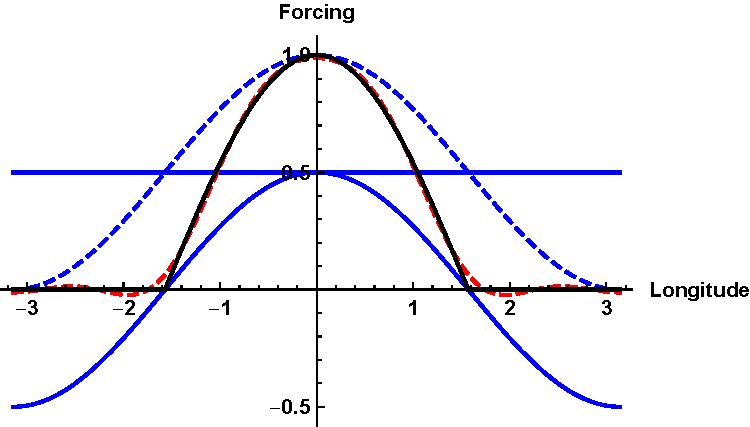
\includegraphics[width=0.7\textwidth]{figures/eqm-zonal-flow/fourier.pdf}
%   \caption{The Fourier series of the realistic forcing.}
%   \label{fig:decomp-forcing}
% \end{figure}



%
%
% The black line in Figure \ref{fig:decomp-forcing} shows the longitudinal form of this radiative equilibrium field on the equator. The red dashed line shows an approximation by a fifth-order Fourier series. The blue dashed line shows the sum of the wave-0 and wave-1 Fourier components (the solid blue lines), which approximates the real field and crucially has a non-zero zonal mean. The first-order term corresponds to the radiative equilibrium field in \citet{showman2011superrotation} -- adding the zeroth-order term adds a non-zero zonal mean.


\subsection{Equilibrium Zonal Flow}

The mechanism in Figure \ref{fig:gierasch} predicts the balance of momentum fluxes that determine the equilibrium state of the zonal flow. At the equator, the horizontal momentum transport from the stationary waves should balance the vertical momentum transport from rising and subsiding air at the substellar and antistellar points. At high latitudes, the horizontal momentum transport from the stationary waves should be balanced by the eastward acceleration of the poleward branch of the meridional circulation. This section will test this prediction in the non-linear shallow-water model.

The zonal-mean momentum equation in a spherical geometry is \citep{showman2011superrotation}:

\begin{equation}\label{eqn:zonal-mean-mom-sphere}
  \begin{split}
    \frac{\partial \overline{u}}{\partial t}=\underbrace{\overline{v}^{*}\left[f-\frac{1}{a \cos \phi} \frac{\partial(\overline{u} \cos \phi)}{\partial \phi}\right]}_{\mathrm{I}}
    \underbrace{-\frac{1}{\overline{h} a \cos ^{2} \phi} \frac{\partial}{\partial \phi}\left[\overline{(h v)^{\prime} u^{\prime}} \cos ^{2} \phi\right]}_{\mathrm{II}} \\
    +\underbrace{\left[\frac{1}{\overline{h}} \overline{u^{\prime} Q^{\prime}}+\overline{R_{u}}^{*}\right]}_{\text { III }} \underbrace{-\frac{\overline{u}^{*}}{\tau_{\mathrm{drag}}}}_{\mathrm{IV}}-\frac{1}{\overline{h}} \frac{\partial\left(\overline{h^{\prime} u^{\prime}}\right)}{\partial t},
  \end{split}
\end{equation}


where $\phi$ is longitude, and all other variables are the same as before. Figure \ref{fig:test-C-accn} shows each of these terms for the steady-state flow in Test C. The ``Mean horizontal'' term is Term I, which produces an acceleration at high latitudes due to the mean meridional velocity. This is primarily balanced by the ``Eddy Horizontal'' flux of Term II, which produces a westward acceleration at high latitudes as it transports eastward momentum towards the equator. This is the balance predicted by Figure \ref{fig:gierasch} and shown in the linear model in Section \ref{sec:lin-sw-grw-results}. There is also a westward acceleration at high latitudes from the ``Vertical Transport'' flux of Term III, as the eastward flow subsides in the descending branch of the meridional circulation. At the equator, the balance is between eastward acceleration due to the ``Eddy Horizontal'' transport from the stationary waves, and westward acceleration due to the ``Vertical Transport'' term discussed in Section \ref{sec:lin-sw-model}. Term I is zero at the equator as there is zero meridional velocity. This agrees with the mechanism in Figure \ref{fig:gierasch} and Section \ref{sec:lin-sw-grw-results}.

\begin{figure}
  \centering
  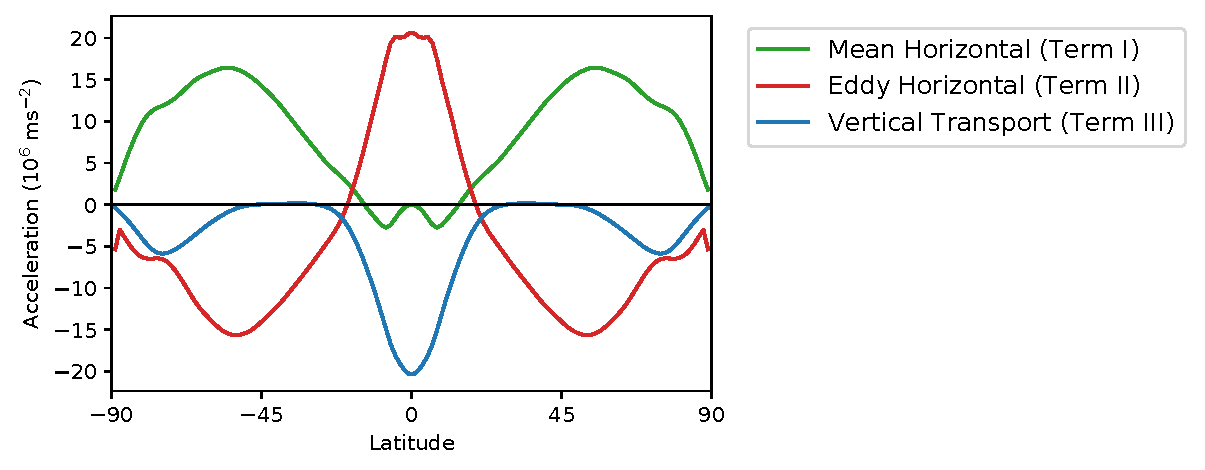
\includegraphics[width=1.0\textwidth]{figures/eqm-zonal-flow/nonlin-balance.pdf}
  \caption{The terms in the zonal-mean zonal momentum equation (Equation \ref{eqn:zonal-mean-mom-sphere}) for Test C with realistic forcing in the non-linear shallow-water model, showing how equilibrium is achieved at the equator and at high latitudes. Note the same balance of forces as in Figures \ref{fig:beta-fluxes-plus-merid} and \ref{fig:accn-terms-jet-level}.}\label{fig:test-C-accn}
\end{figure}


These non-linear shallow-water simulations have shown how the sinusoidal day-night forcing produces an equatorward momentum transport, how a non-zero zonal-mean forcing produces a meridional circulation, and how a realistic forcing combines these processes to drive the GRW mechanism. The realistic forcing field in Test C produces eastward flow at all latitudes, matching the GCM simulations that could not be explained by the model with sinusoidal day-night forcing. The balance of momentum fluxes at the equator and at high latitudes matched the balance predicted by the GRW mechanism. In the next section, I will show this is also the case in idealised GCM simulations of the atmosphere of a tidally locked planet.


% At the equator, the horizontal stationary momentum flux (Term II) balances the vertical stationary momentum flux (Term III). At high latitudes, the horizontal mean momentum flux (Term I) balances the horizontal stationary momentum flux (Term II).


%
% In the next section, I will apply  the GRW mechanism to predict scaling relations for the zonal flow in the non-linear shallow-water model and the GCM.





% \begin{figure}
%   \centering
%   \begin{subfigure}[t]{0.32\textwidth}
%     \includegraphics[width=1.0\textwidth]{figures/eqm-zonal-flow/test-1-accn.pdf}
%     \caption{1}
%     \label{fig:test-1-accn}
%   \end{subfigure}
%   %
%   \begin{subfigure}[t]{0.32\textwidth}
%     \includegraphics[width=1.0\textwidth]{figures/eqm-zonal-flow/test-2-accn.pdf}
%     \caption{2}
%     \label{fig:test-2-accn}
%   \end{subfigure}
%   %
%   \begin{subfigure}[t]{0.32\textwidth}
%     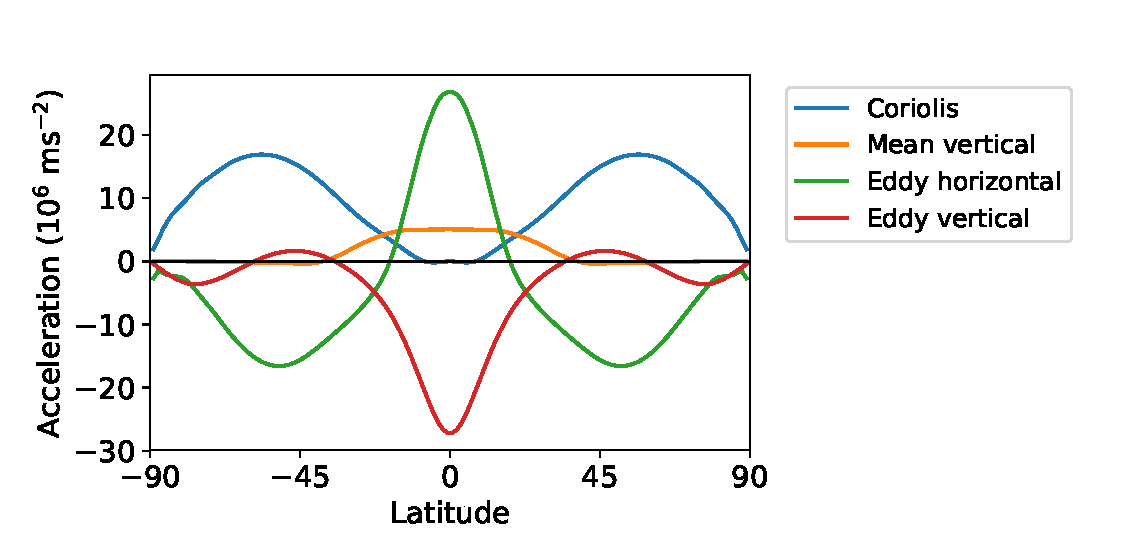
\includegraphics[width=1.0\textwidth]{figures/eqm-zonal-flow/test-3-accn.pdf}
%     \caption{3}
%     \label{fig:test-3-accn}
%   \end{subfigure}
%   \caption{Accelerations.}
%   \label{fig:nonlin-tests-accn}
% \end{figure}


%SECTION CONCLUSIONS

\section{GCM Simulations of the GRW Mechanism}\label{sec:gcm-sim-grw}

This section shows the formation of zonal flow in the GCM Exo-FMS. I will compare an idealised simulation of a tidally locked planet to a simulation of an asynchronously rotating planet, and show that the balance of momentum fluxes in the GCM is same as the shallow-water models in the previous section. The next section will use this mechanism to predict the scaling behaviour of the zonal flow in a suite of tests in the non-linear shallow-water model and the GCM.

Test 1 is a tidally locked planet with a pure $N_{2}$ atmosphere with radius  $1.0\ R_{E}$, rotation rate $\Omega_{E}/10$, surface pressure $\SI{1}{\bar}$, longwave optical thickness $1.0$, shortwave optical thickness $0.0$, and instellation $\SI{1000}{\watt\per\metre\squared}$. This test is an idealised, general example of a tidally locked terrestrial planet orbiting an M-dwarf, using Exo-FMS with semi-grey radiative transfer and dry convective adjustment.

Figure \ref{fig:default-gcm-temp} shows the equilibrium global circulation of Test 1, time-averaged from 1000 to 2000 days of the simulation. The global temperature and wind fields show the typical superrotating jet and hot-spot shift seen on tidally locked planets \citep{showman2012review, pierrehumbert2018review}. The zonal-mean zonal wind is dominated by a single equatorial jet, which is shown in Chapter \ref{ch:wave-mean-flow} to produce the hot-spot shift by shifting the stationary planetary waves eastward. Note that there is prograde eastward flow at all latitudes of the jet in this test, which is the situation that this chapter aims to explain.

Test 2 is an asynchronously rotating planet with otherwise the same properties as Test 1. Its instellation is zonally uniform but has the same zonal-mean instellation as Test 1. I will show that this produces the same meridional circulation on the first day of the test when the response to forcing is small and linear. Figure \ref{fig:default-gcm-axi-example} shows the global circulation of the equilibrium state of Test 2, time-averaged from 1000 to 2000 days of the simulation. This atmosphere has an zonally uniform temperature field, and two subtropical jets produced by its meridional circulation. Its ``Hadley'' cells are global due to its 10 day rotation period, unlike the more rapidly rotating Earth with its multiple cells.

 These two tests will show how the meridional circulation on a tidally locked planet produces subtropical jets before the stationary waves from the day-night forcing produce equatorial acceleration, as described by the GRW mechanism. \citet{norton2006tropical} used similar simulations to these two tests to show the formation of superrotation by tropical heating on the Earth.

\begin{figure}
  \centering
  \begin{subfigure}[t]{0.48\textwidth}
    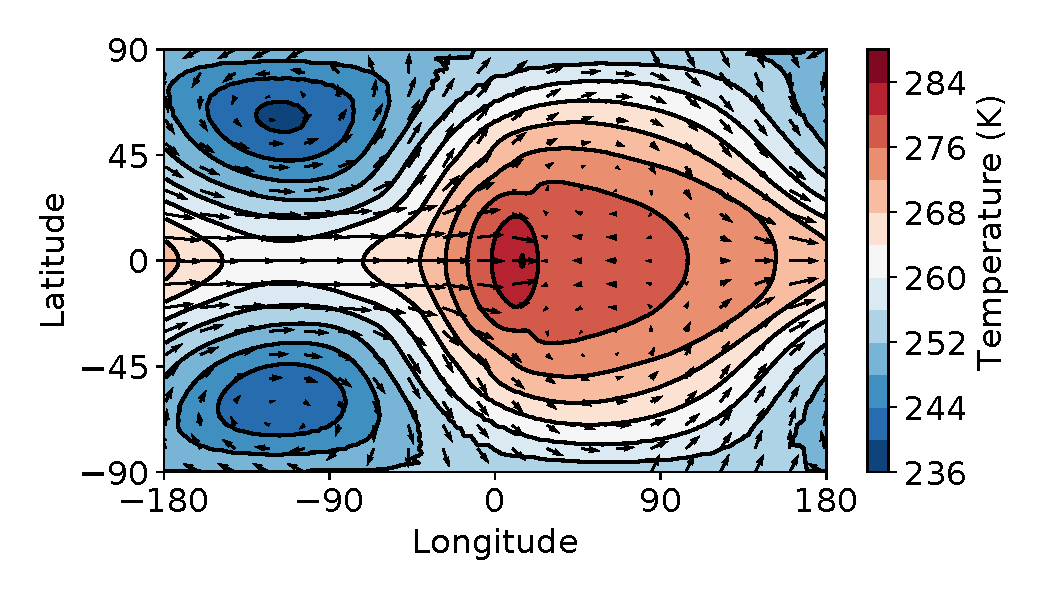
\includegraphics[width=1.0\textwidth]{figures/eqm-zonal-flow/default-gcm-temp.pdf}
    \caption{Temperature and velocity fields.}\label{fig:default-gcm-temp}
  \end{subfigure}
\quad
  \begin{subfigure}[t]{0.48\textwidth}
    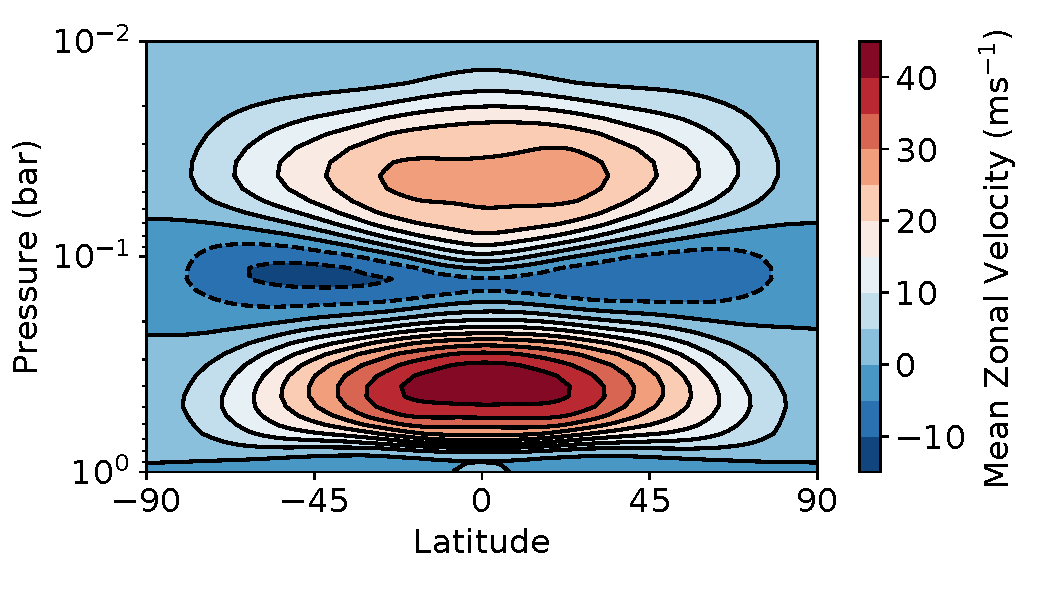
\includegraphics[width=1.0\textwidth]{figures/eqm-zonal-flow/default-gcm-zonal-flow.pdf}
    \caption{Zonal-mean zonal velocity.}\label{default-gcm-zonal-flow}
  \end{subfigure}
  \caption{The global circulation of Test 1, time-averaged from 1000 to 2000 days of the simulation. The temperature field is at the half-surface pressure level. This is a typical tidally locked Earth-sized planet, with prograde zonal flow at all latitudes at the level of maximum jet flow.}\label{fig:default-gcm-example}
\end{figure}


\begin{figure}
  \centering
  \begin{subfigure}[t]{0.48\textwidth}
    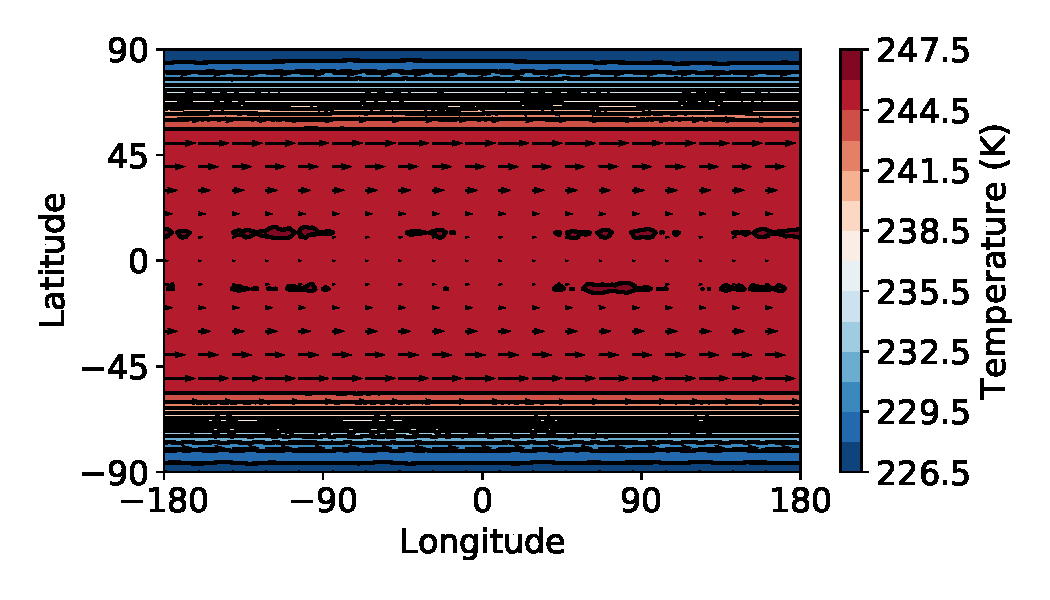
\includegraphics[width=1.0\textwidth]{figures/eqm-zonal-flow/default-gcm-axi-temp.pdf}
    \caption{Temperature and velocity fields.}\label{fig:default-gcm-axi-temp}
  \end{subfigure}
\quad
  \begin{subfigure}[t]{0.48\textwidth}
    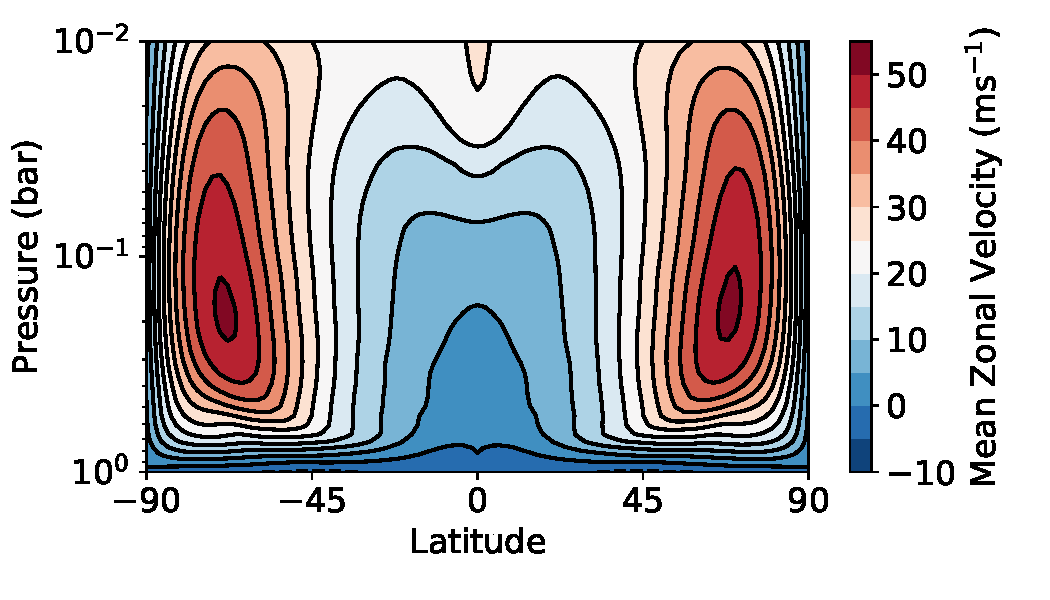
\includegraphics[width=1.0\textwidth]{figures/eqm-zonal-flow/default-gcm-axi-zonal-flow.pdf}
    \caption{Zonal-mean zonal velocity.}\label{default-gcm-axi-zonal-flow}
  \end{subfigure}
  \caption{The global circulation of Test 2, time-averaged from 1000 to 2000 days of the simulation. The temperature field is at the half-surface pressure level. This is an idealised asynchronously rotating Earth-sized planet, with subtropical jets formed by the mean meridional circulation.}\label{fig:default-gcm-axi-example}
\end{figure}


\subsection{Initial Meridional Circulation}

Section \ref{sec:grw-on-tl} suggested that the meridional circulation on a tidally locked planet primarily depends on the zonal mean of the instellation. This means that the longitudinal variation of the instellation and circulation does not greatly affect the GRW mechanism. Figure \ref{fig:day-1-tide-axi} shows that this is true for the early stages of Tests 1 and 2, when the response to forcing is small and linear. The first column shows the zonal velocity in the first day at the surface of each test, where Test 1 has diverging flow from the substellar point and Test 2 has weak surface westerlies forming as part of a meridional circulation.

The second column shows the zonal-mean zonal velocity on the first day. The two tests have almost exactly the same zonal-mean zonal velocity, despite their different longitudinal variation. The third column shows that they also have almost the same streamfunction. This supports the argument in Section \ref{sec:grw-on-tl} that only the zonal mean of the forcing (the same in Tests 1 and 2) affects the zonal-mean meridional circulation in the linear limit of weak forcing. The meridional circulation only enters the zonal-mean zonal momentum equation \citep{showman2011superrotation} as a zonal-mean quantity, so the GRW mechanism can be applied to the zonal-mean circulation without considering the actual longitudinal variation of the instellation. In reality, as each test spins up the assumption of linearity will become less accurate as the perturbations increase and the zonal flow affects the meridional circulation.

These tests support the use of the GRW mechanism to explain the formation of zonal flow on tidally locked planets. They show that the meridional circulation primarily affects the zonal flow through its zonal mean only. The next section will show how the equatorward momentum transport on tidally locked planets modifies the subtropical jets and produces equatorial superrotation.



%
% It shows the time-mean results of the first day of spin-up of these simulations from rest, where the response to the applied forcing is still small and linear. The leftmost panels show the highly different zonal winds at the surface of the tidally locked Test 1, and the surface of the axisymmetric Test 2. However, the next panels are the zonal mean zonal-wind of each test, showing the identical subtropical jets beginning to be formed by the mean meridional circulation in each case. These are the same due to the linearity demonstrated above -- the mean meridional circulation only depends on the zonal mean of the forcing, which is the same in Tests 1 and 2. The final panels show the same effect -- each test has the same zonal-mean mass streamfunction, as the meridional circulation is the same.
%
% This means that the effect of the mean meridional circulation on the zonal mean momentum equation (through term I in Equation \ref{eqn:zonal-mean-mom}) is the same in the tidally locked Test 1 as in the axisymmetric Test 2.


\begin{figure}
  \centering

  \begin{subfigure}[t]{0.31\textwidth}
    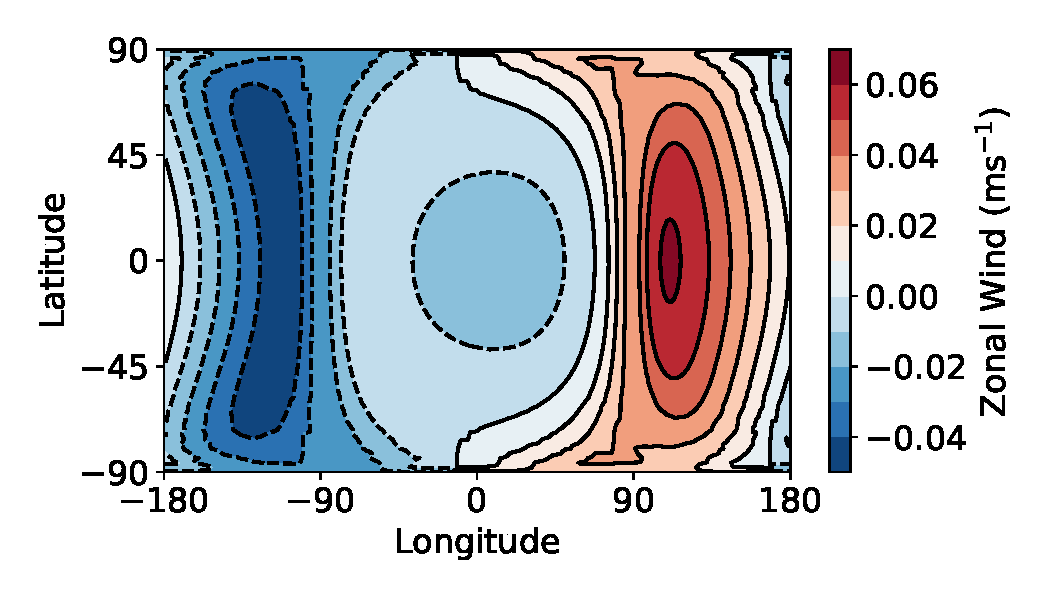
\includegraphics[width=\textwidth]{figures/eqm-zonal-flow/zonal-wind-map-tide-day1.pdf}
    \caption{1: Surface zonal velocity.}
  \end{subfigure}
\enskip
  \begin{subfigure}[t]{0.31\textwidth}
    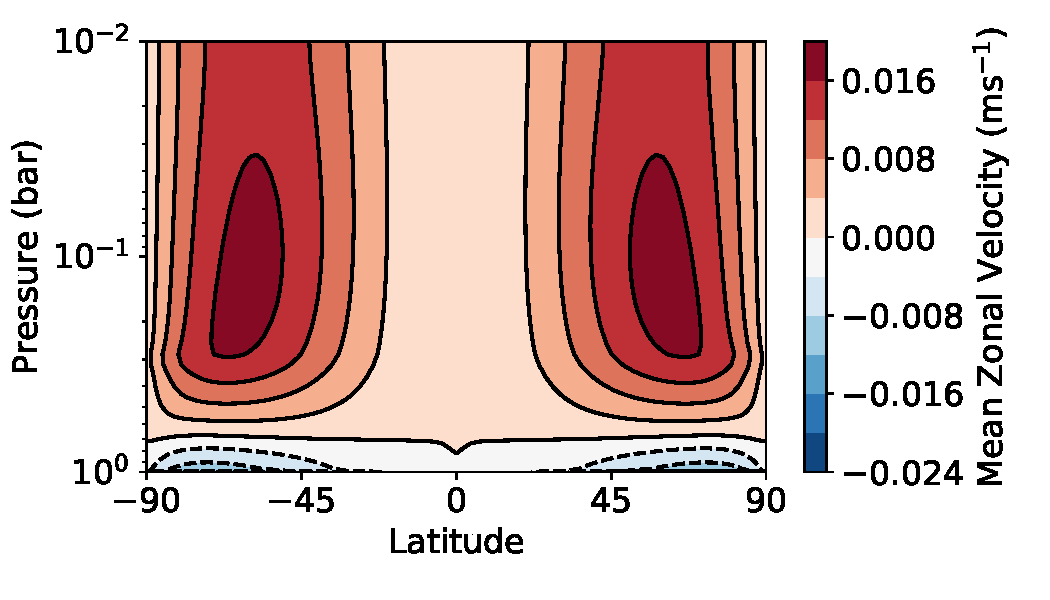
\includegraphics[width=\textwidth]{figures/eqm-zonal-flow/zonal-wind-tide-day1.pdf}
    \caption{1: Zonal velocity.}
  \end{subfigure}
\enskip
  \begin{subfigure}[t]{0.31\textwidth}
    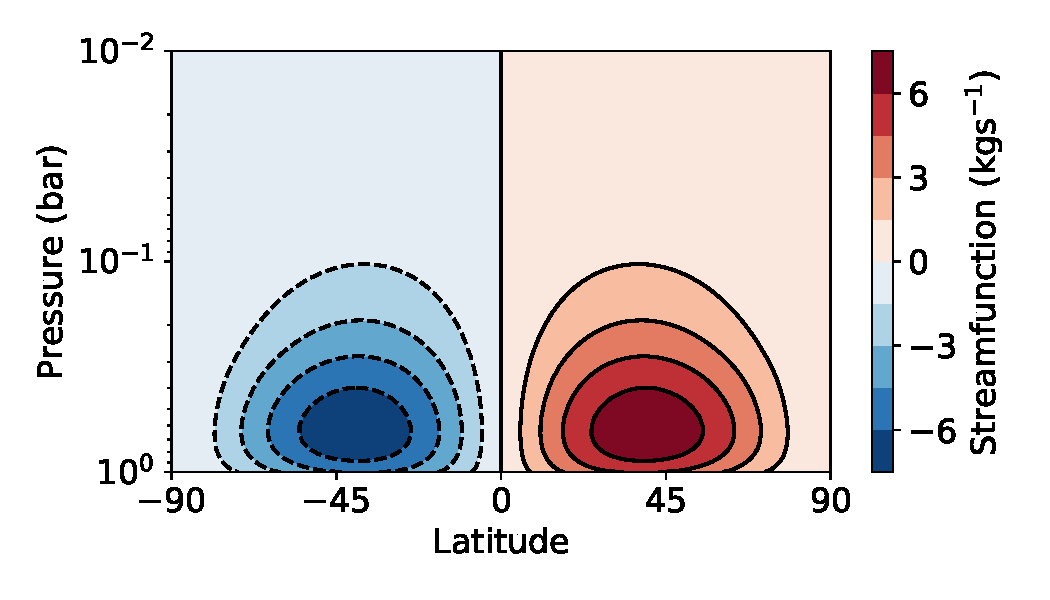
\includegraphics[width=\textwidth]{figures/eqm-zonal-flow/streamfunction-tide-day1.pdf}
    \caption{1: Mass streamfunction.}
  \end{subfigure}
  \\
  \begin{subfigure}[t]{0.31\textwidth}
    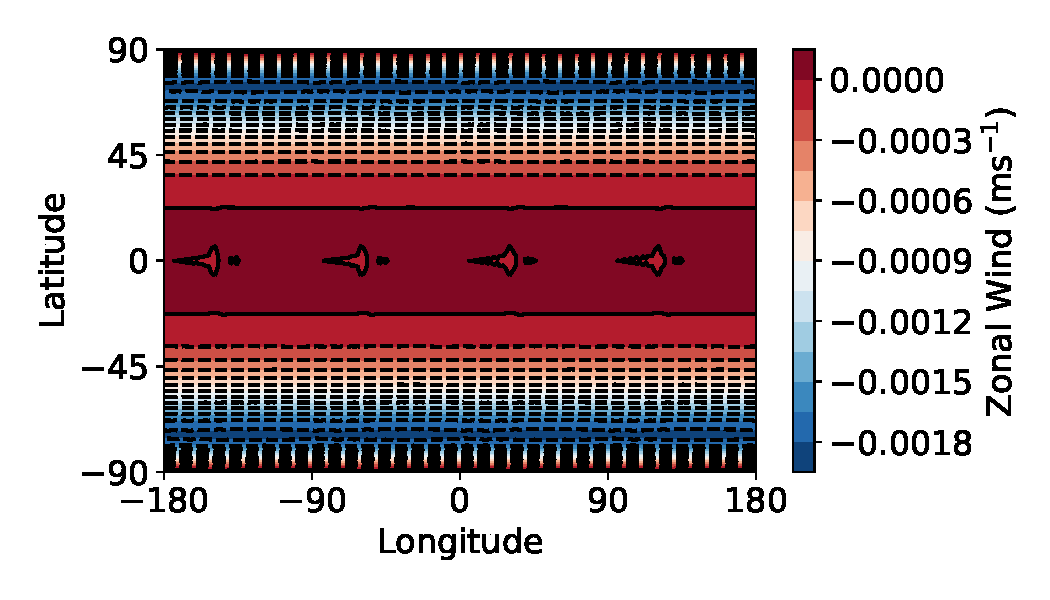
\includegraphics[width=\textwidth]{figures/eqm-zonal-flow/zonal-wind-map-axi-day1.pdf}
    \caption{2: Surface zonal velocity.}
  \end{subfigure}
\enskip
  \begin{subfigure}[t]{0.31\textwidth}
    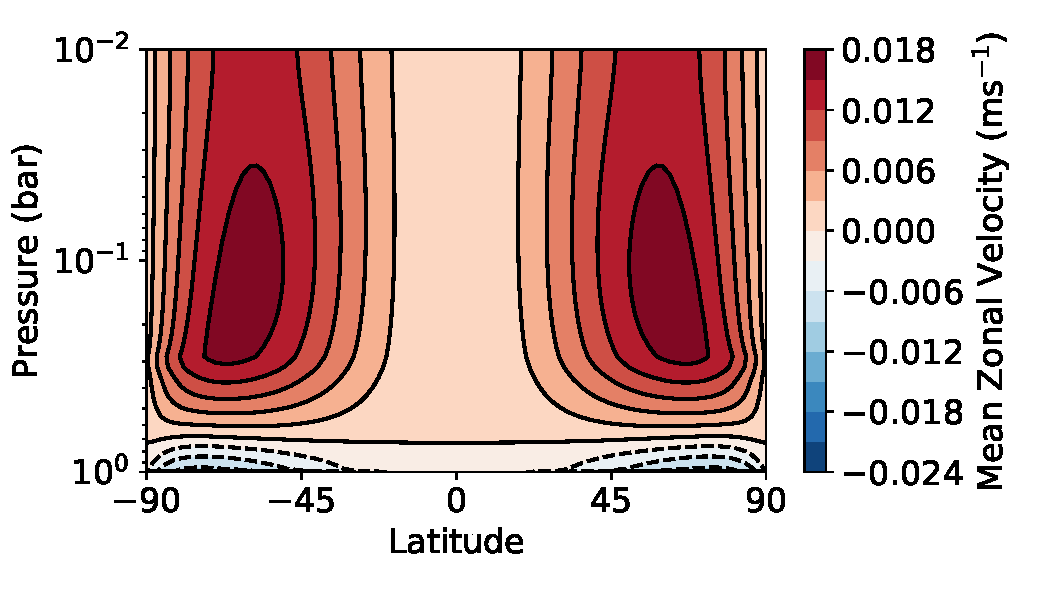
\includegraphics[width=\textwidth]{figures/eqm-zonal-flow/zonal-wind-axi-day1.pdf}
    \caption{2: Zonal velocity.}
  \end{subfigure}
\enskip
  \begin{subfigure}[t]{0.31\textwidth}
    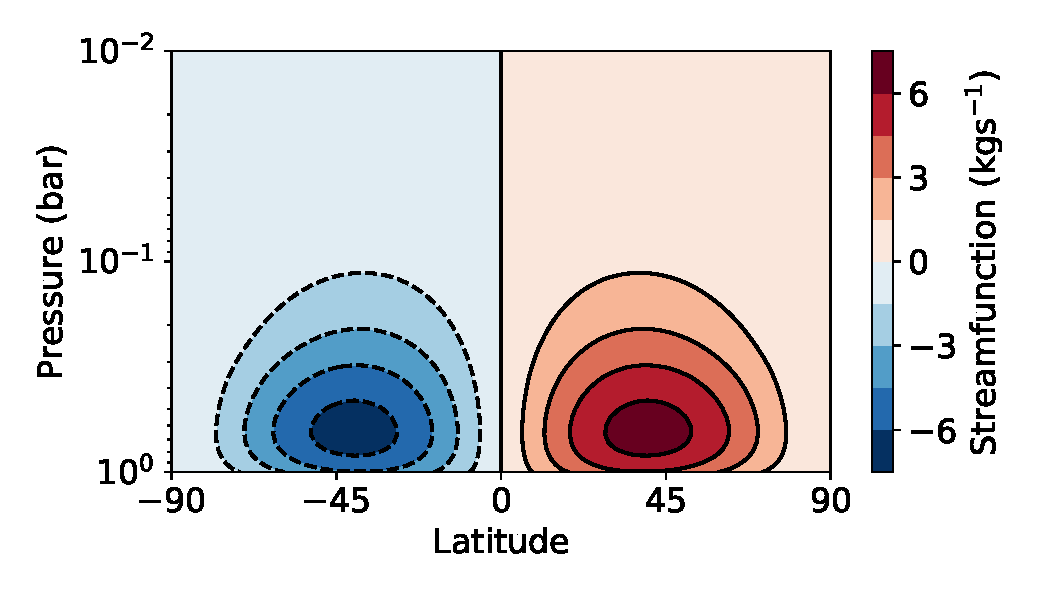
\includegraphics[width=\textwidth]{figures/eqm-zonal-flow/streamfunction-axi-day1.pdf}
    \caption{2: Mass streamfunction.}
  \end{subfigure}
  \caption{Time-mean results from Tests 1 and 2, for the first day after initialisation from rest. The top row shows the tidally locked planet Test 1, and the bottom row shows Test 2, a planet with axisymmetric forcing with the same zonal mean. The zonal mean zonal velocity and mean mass streamfunction are the same in both cases, despite the large differences in the longitudinal distribution of the forcing.}\label{fig:day-1-tide-axi}
\end{figure}



% Following REF(ZG), I impose a background flow $\overline{U}(\phi)$ based on the vorticity profile X.

% Then I linearise the equations X about this flow and calculate the response to forcing X with the method X in Appendix X, then calculate the resulting zonal acceleration from Equation X.

% Figure X shows the solution with an imposed jet X that gives zero zonal acceleration at the equator, with and without the background flow from a mean meridional circulation X. It shows that with the mean meridional circulation, the flow can be prograde at all latitudes (although must be sub-rotating at high latitudes).
%
% Figure X shows a strong meridional circulation with dominant subtropical jets. The pattern matches the circulation in Noda, with two peaks off the equator.




%SUBSECTION -- DEMONSTRATION OF MECHANISM
\subsection{Demonstration of GRW Mechanism}


This section shows the formation of zonal flow in Tests 1 and 2, demonstrating how the GRW mechanism adds angular momentum to the atmosphere in Test 1 and creates eastward flow at all latitudes. The total atmospheric angular momentum is \citep{lebonnois2012momentum}:

\begin{equation}
  M=\int_{V} u a \cos \theta d m
\end{equation}

where $\int_{V}$ is the integral of mass over the whole atmosphere, $u$ is the local zonal velocity, $a$ is the planetary radius, and $\theta$ is the latitude.

Figure \ref{fig:global-m} shows the total atmospheric angular momentum in Test 1 as it spins up from rest. The only source or sink of angular momentum apart from numerical error is the linear Rayleigh drag applied to the winds in the boundary layer near the surface. It gains angular momentum as the surface drags the winds in the boundary layer, then reaches equilibrium when there is sufficient eastward wind and westward torque for no net effect. The total angular momentum varies over a period of hundreds of days, with fluctuations that are small compared to the large variability in the angular momentum of similar simulations of superrotation on Venus \citep{lebonnois2012momentum}.

% Test 1 reaches equilibrium at a greater total angular momentum than Test 2, which may be due to the equatorward momentum transport reducing the eastward momentum transported to the surface by the meridional circulation, so allowing a greater eastward flow in the upper branch before the boundary layer winds reach zero net drag.

Figure \ref{jet-layer-m} shows the angular momentum in Test 1 in the model level of the maximum zonal-mean zonal flow. The angular momentum in this level increases as the model spins up, then reaches a positive value at equilibrium. This contradicts the shallow-water model in \citet{showman2011superrotation} which loses angular momentum from the level of the jet. The positive net angular momentum is explained by the GRW mechanism, which transports angular momentum from the surface to the atmosphere, and to the upper branch of the meridional circulation.

\begin{figure}
  \centering
  \begin{subfigure}[t]{0.48\textwidth}
    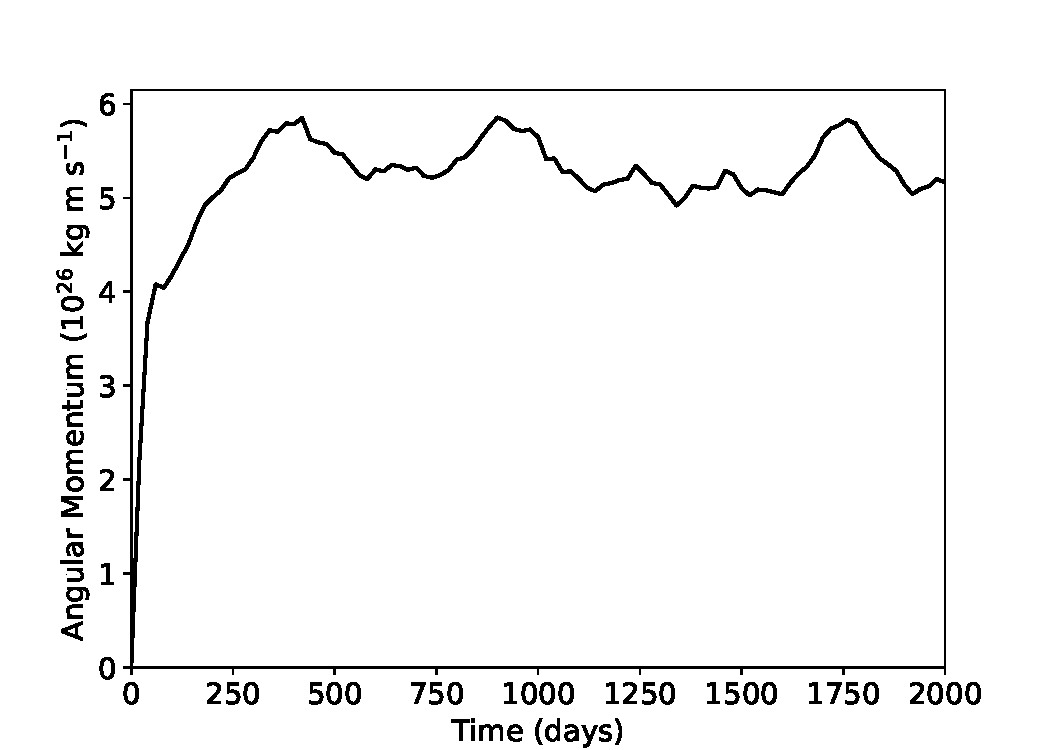
\includegraphics[width=1.0\textwidth]{figures/eqm-zonal-flow/global-m.pdf}
    \caption{Total angular momentum.}\label{fig:global-m}
  \end{subfigure}
\quad
  \begin{subfigure}[t]{0.48\textwidth}
    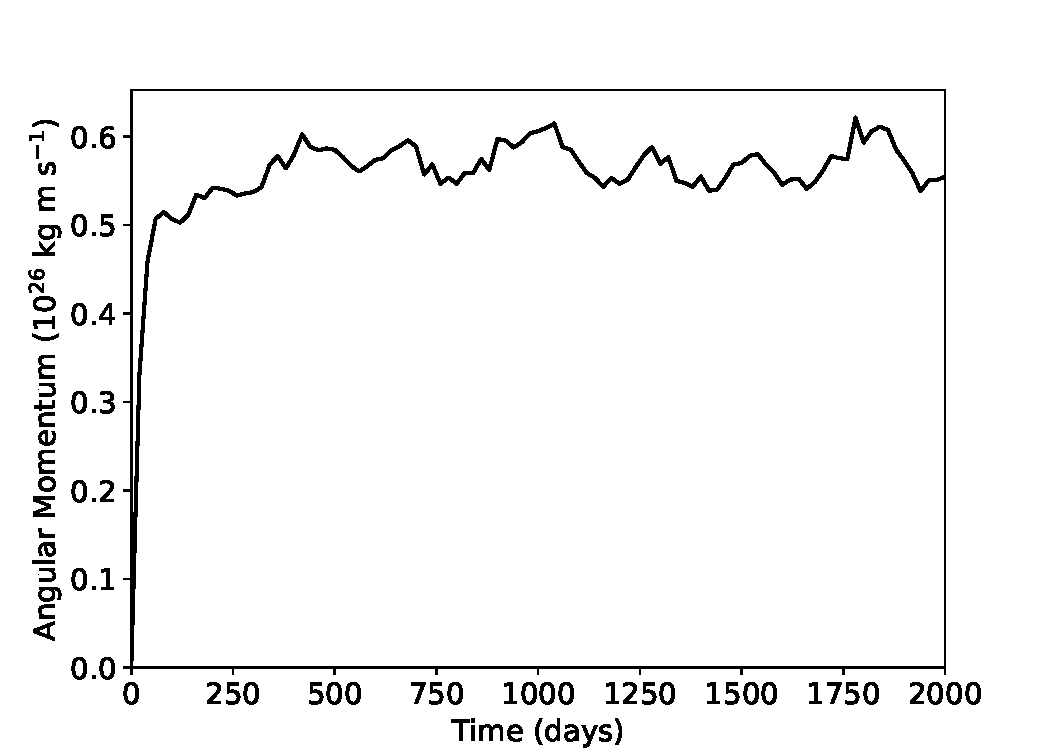
\includegraphics[width=1.0\textwidth]{figures/eqm-zonal-flow/jet-layer-m.pdf}
    \caption{Angular momentum in the jet layer.}\label{jet-layer-m}
  \end{subfigure}
  \caption{The spin-up in Test 1 of angular momentum globally and at the pressure level where the jet is strongest, showing how both regions gain momentum over time then equilibrate.}\label{fig:global-jet-layer-m-spinup}
\end{figure}

Figures \ref{fig:test-1-spinup} and \ref{fig:test-2-spinup} show the development of the zonal flow in Tests 1 and 2. Figure \ref{fig:test-2-spinup} shows the evolution of the flow in Test 2, where subtropical jets form immediately due to the mean meridional circulation, then strengthen and reach equilibrium. Figure \ref{fig:test-1-spinup} shows that the same subtropical jets form initially in Test 1, but then the stationary waves transport angular momentum towards the equator \citep{showman2011superrotation}. Test 1 reaches an equilibrium state with a single equatorial jet and eastward flow at high latitudes due to acceleration from the meridional circulation.



% The first row of Figure \ref{fig:test-1-2-spinup} shows the development of the zonal-mean zonal wind as it spins up from rest in the axisymmetric case, Test 2. The forcing gradient between the equator and the pole results in a mean meridional circulation that rapidly produces subtropical jets, which strengthen with time until they reach equilibrium. Note that there is no eastward flow at the equator, and the superrotation index is negative everywhere as there is no process to transport momentum equatorward.
%
% The second row of Figure \ref{fig:test-1-2-spinup} shows the development of the zonal-mean zonal wind as it spins up from rest in the tidally locked case, Test 1. The first panel shows that exactly the same subtropical jets form at the start of the spin-up as in the axisymmetric case, due to the linear response as explained previously. In the next panel, the stationary waves induced by the stationary forcing transport momentum towards the equator, producing eastward superrotating flow there. This weakens the subtropical jets, but they are still present at high latitudes. In the final panel, the equatorward transport has produced a strong single equatorial jet, with no distinct subtropical jets present. The balance between these the equatorward transport and the mean meridional circulation determines the relative strength of the equatorial and subtropical jets, which I will investigate in more detail later.

\begin{figure}
  \centering
  \begin{subfigure}[t]{0.31\textwidth}
    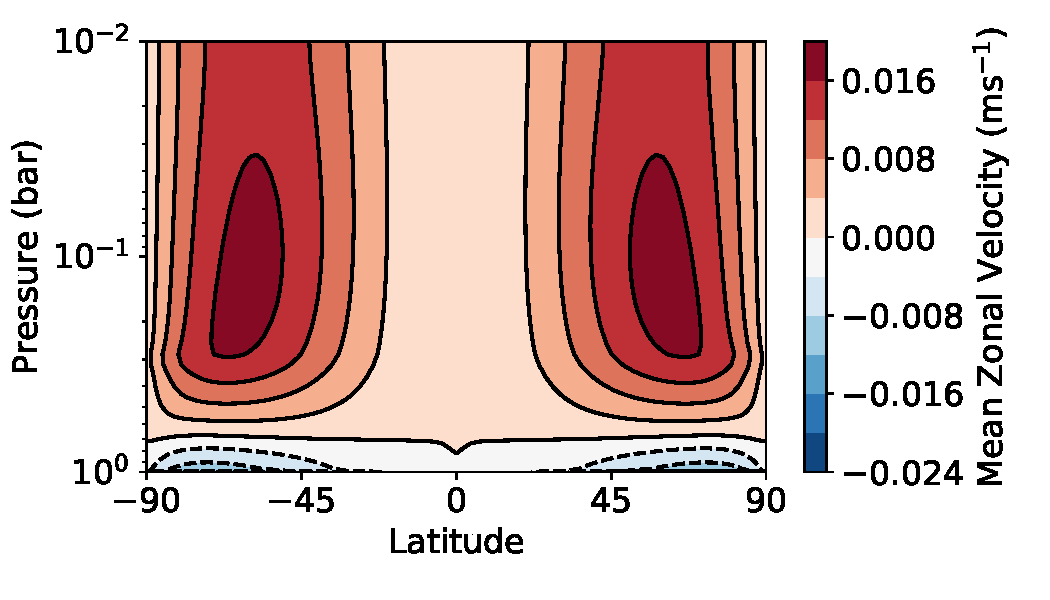
\includegraphics[width=\textwidth]{figures/eqm-zonal-flow/zonal-wind-tide-day1.pdf}
    \caption{Day 1.}
  \end{subfigure}
\enskip
  \begin{subfigure}[t]{0.31\textwidth}
    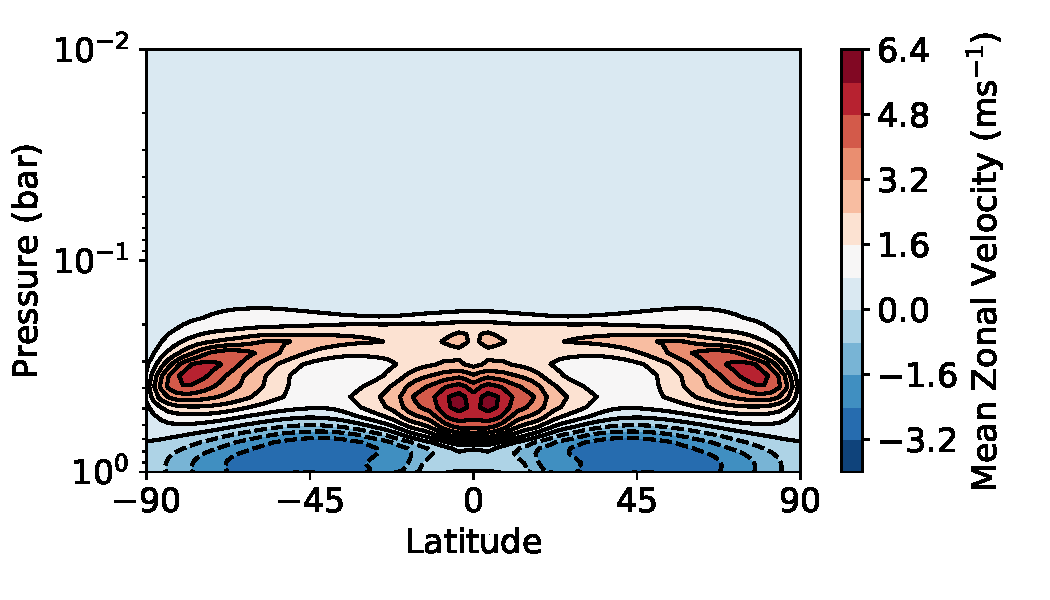
\includegraphics[width=\textwidth]{figures/eqm-zonal-flow/tl-zonal-u-5day.pdf}
    \caption{Day 5.}
  \end{subfigure}
\enskip
  \begin{subfigure}[t]{0.31\textwidth}
    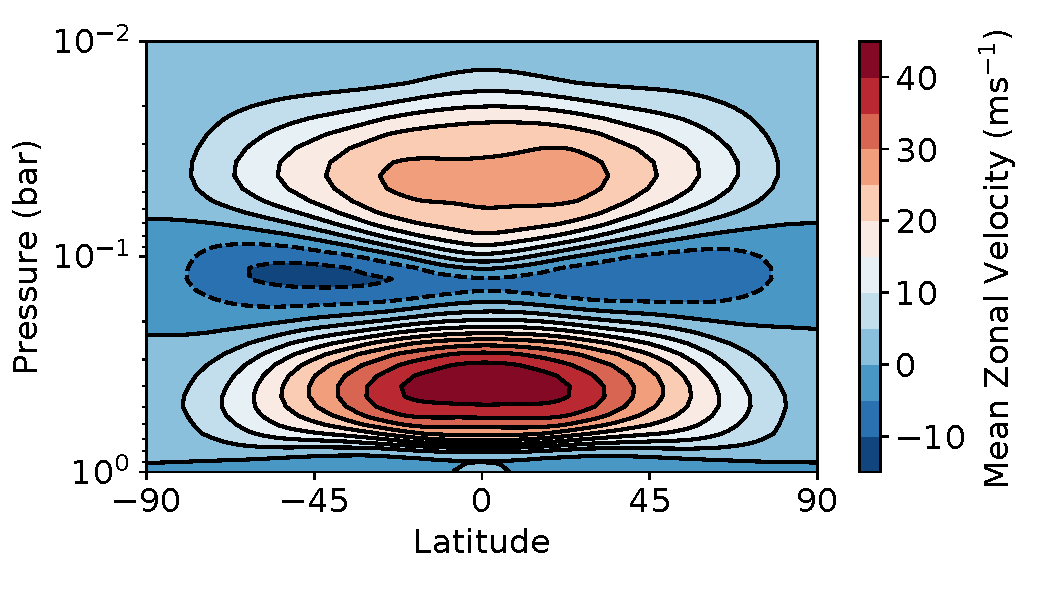
\includegraphics[width=1.0\textwidth]{figures/eqm-zonal-flow/default-gcm-zonal-flow.pdf}
    \caption{1000 to 2000 days.}
  \end{subfigure}
  \caption{The zonal-mean zonal velocity of the tidally locked planet in Test 1 as it spins up from rest, forming subtropical jets before the equatorward momentum transport produces the equatorial jet. The time-mean fields on day 1, on day 5, and from day 1000 to 2000 are plotted.}\label{fig:test-1-spinup}
\end{figure}


\begin{figure}
  \centering
  \begin{subfigure}[t]{0.31\textwidth}
    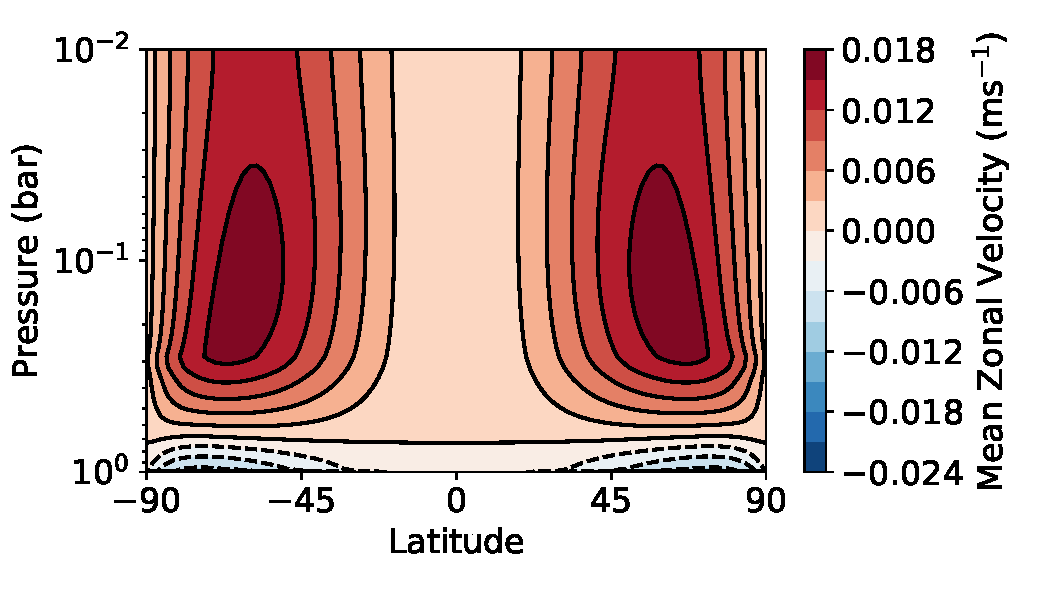
\includegraphics[width=\textwidth]{figures/eqm-zonal-flow/zonal-wind-axi-day1.pdf}
    \caption{Day 1.}
  \end{subfigure}
\enskip
  \begin{subfigure}[t]{0.31\textwidth}
    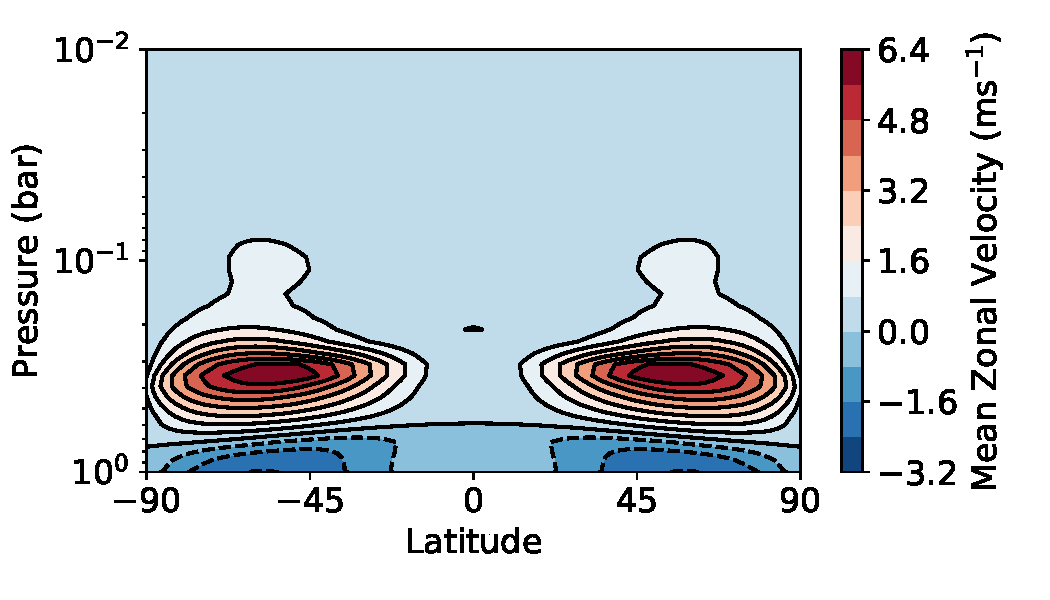
\includegraphics[width=\textwidth]{figures/eqm-zonal-flow/axi-zonal-u-5day.pdf}
    \caption{Day 5.}
  \end{subfigure}
\enskip
  \begin{subfigure}[t]{0.31\textwidth}
    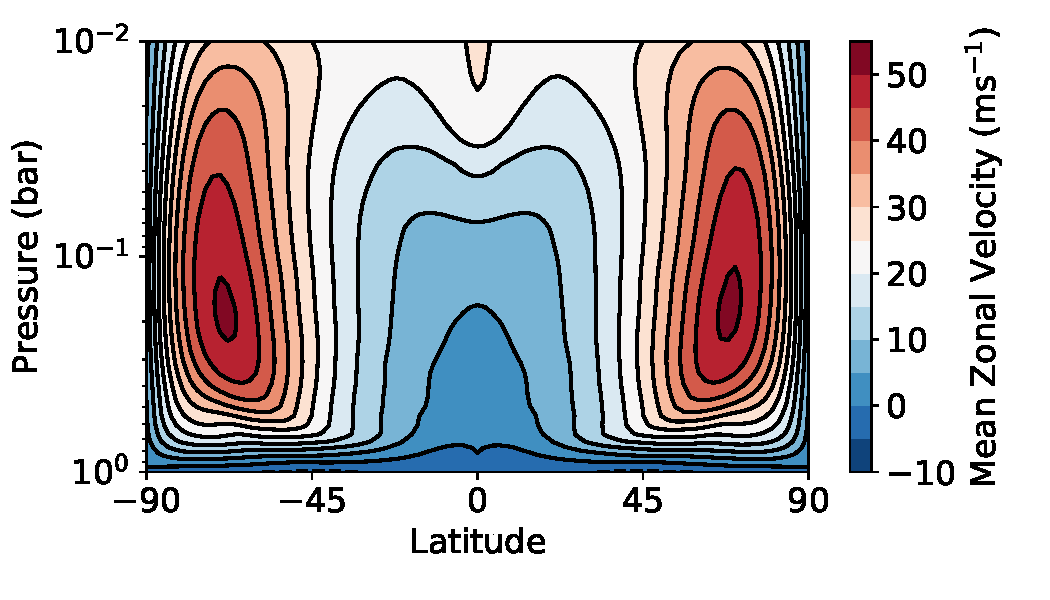
\includegraphics[width=1.0\textwidth]{figures/eqm-zonal-flow/default-gcm-axi-zonal-flow.pdf}
    \caption{1000 to 2000 days.}
  \end{subfigure}
  \caption{The zonal-mean zonal velocity of the axisymmetrically forced planet in Test 2 as it spins up from rest, forming subtropical jets. The time-mean fields on day 1, on day 5, and from day 1000 to 2000 are plotted.}\label{fig:test-2-spinup}
\end{figure}



%
% Figure \ref{fig:default-gcm-velocity-drag} shows the time-mean zonal-mean zonal velocity and the resulting drag for Test 1 from 500 to 1500 days (the same as the final panel of \ref{fig:test-1-2-spinup}). The second panel shows the effect of the linear Rayleigh drag applied in the boundary layer, which decays linearly with pressure away from the surface to zero at $70 \%$ of the surface pressure. There is a positive westerly acceleration due to drag at the surface due to the surface easterlies formed by the mean meridional circulation. This drag pumps prograde momentum into the atmosphere, which is responsible for the increase in angular momentum during spin-up shown by Figure \ref{fig:global-jet-layer-m-spinup}.



\subsection{Zonal Momentum Fluxes}

This section shows that the GRW mechanism explains the equilibrium zonal momentum budget in Test 1. The steady-state zonal-mean momentum equation is \citep{lutsko2018response}:

\begin{equation}\label{eqn:zonal-mean-mom-gcm}
  \begin{split}
    \frac{\partial \overline{u}}{\partial t} = \underbrace{f[\overline{v}]-\frac{[\overline{v}]}{a \cos \phi} \frac{\partial}{\partial \phi}([\overline{u}] \cos \phi)}_{Ia}
    \underbrace{-[\overline{\omega}] \frac{\partial[\overline{u}]}{\partial p}}_{Ib} \\
    \underbrace{-\frac{1}{a \cos ^{2} \phi} \frac{\partial}{\partial \phi}\left(\left[\overline{u}^{\prime} \overline{v}^{\prime}\right] \cos ^{2} \phi\right)}_{IIa}
    \underbrace{-\frac{\partial}{\partial p}\left[\overline{u}^{\prime} \overline{\omega}^{\prime}\right]}_{IIb}
    \underbrace{+\left[\overline{F_{x}}\right]}_{III} \end{split}
\end{equation}

where $\omega$ is the vertical velocity, and all other variables are the same as before. Terms Ia and Ib are the mean horizontal and vertical momentum transport due to the mean meridional circulation. Term IIa is the eddy horizontal momentum transport from the stationary wave response to the stellar forcing, and Term IIb is the eddy vertical momentum transport due to vertical motion. This vertical motion is mostly due to air rising at the substellar point and subsiding on the night-side. Term III is the forcing applied to the zonal winds, which in this case is the Rayleigh drag in the boundary layer near the surface.

Figure \ref{fig:default-gcm-accelerations} shows each of the momentum transport terms in Equation \ref{eqn:zonal-mean-mom-gcm}. Term Ia is plotted in Figure \ref{fig:mean-horiz}, which shows how the mean meridional circulation produces an acceleration in the midlatitudes in its poleward branch and has no effect at the equator. There is a westward acceleration at the surface due to the lower branch of the mean meridional circulation. This produces the westward surface flow that results in an eastward torque on the atmosphere from the Rayleigh drag in the boundary layer.

Figure \ref{fig:mean-vert} shows Term Ib, where the primary effect is the ascending branch of the mean meridional circulation moving the equatorial jet upwards, as shown by the deceleration below the centre of the jet and the acceleration above the centre of the jet. This term has zero effect where there is zero vertical gradient in the mean zonal flow, so it does not affect the maximum zonal flow at the centre of the jet, and is not as important as the other terms to the equilibrium state.

Figure \ref{fig:stat-horiz} plots Term IIa, and shows how the stationary waves excited by the stellar forcing transport eastward momentum horizontally towards the equator. This produces an acceleration at the equator and a deceleration at higher latitudes. Term IIb in Figure \ref{fig:stat-vert} shows how the vertical momentum transport decelerates the jet. It moves stationary air up on the day-side, reducing the specific westerly angular momentum of the jet. There is an additional deceleration on the jet from the subsiding air on the night-side moving eastward angular momentum down and out of the jet layer. This produces eastward flow at the surface, which results in a westward drag that opposes the eastward drag on the lower branch of the meridional circulation, resulting eventually in equilibrium.


Figure \ref{fig:accn-terms-jet-level} shows each term in Figure \ref{fig:default-gcm-accelerations} at \SI{0.3}{\bar}, near the centre of the jet. It shows that the Terms Ia and IIa balance at high latitudes, and that Term IIb balances Term IIa at the equator, as shown in the linear model in Figure \ref{fig:beta-fluxes-plus-merid}. Terms Ia and IIa become weak at very high latitudes, unlike the shallow-water model in Figure \ref{fig:test-C-accn} where both terms are strong almost until the pole. This is because the meridional circulation does not extend all the way to the pole in the GCM, unlike in the idealised shallow-water model. The balance of fluxes governing the equilibrium flow is still the same in both models.

\begin{figure}
  \centering
  \begin{subfigure}[t]{0.48\textwidth}
    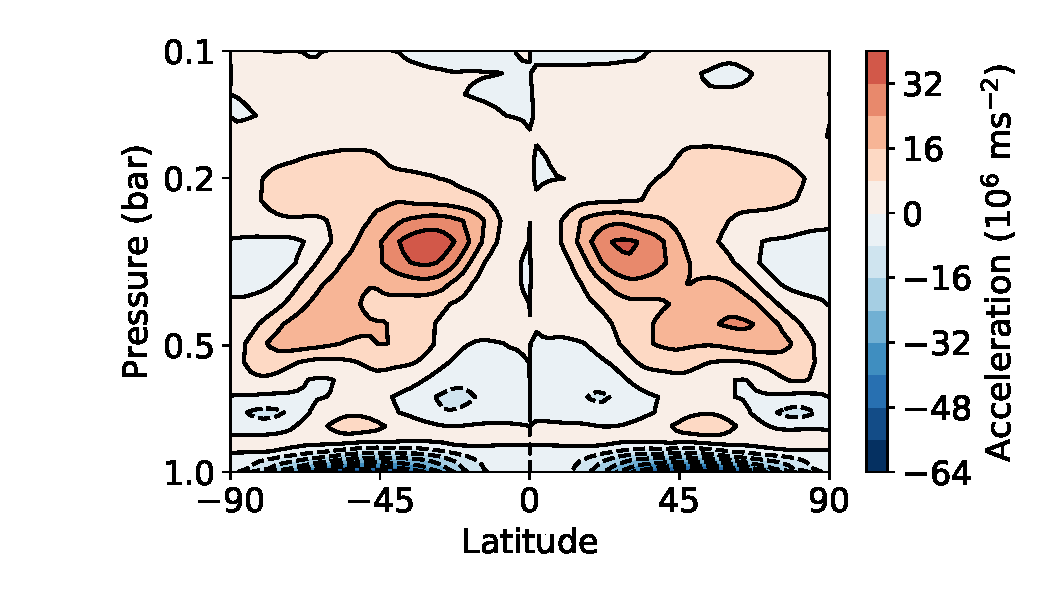
\includegraphics[width=\textwidth]{figures/eqm-zonal-flow/0_flux.pdf}
    \caption{Term Ia, Mean Horizontal.}\label{fig:mean-horiz}
  \end{subfigure}
\quad
  \begin{subfigure}[t]{0.48\textwidth}
    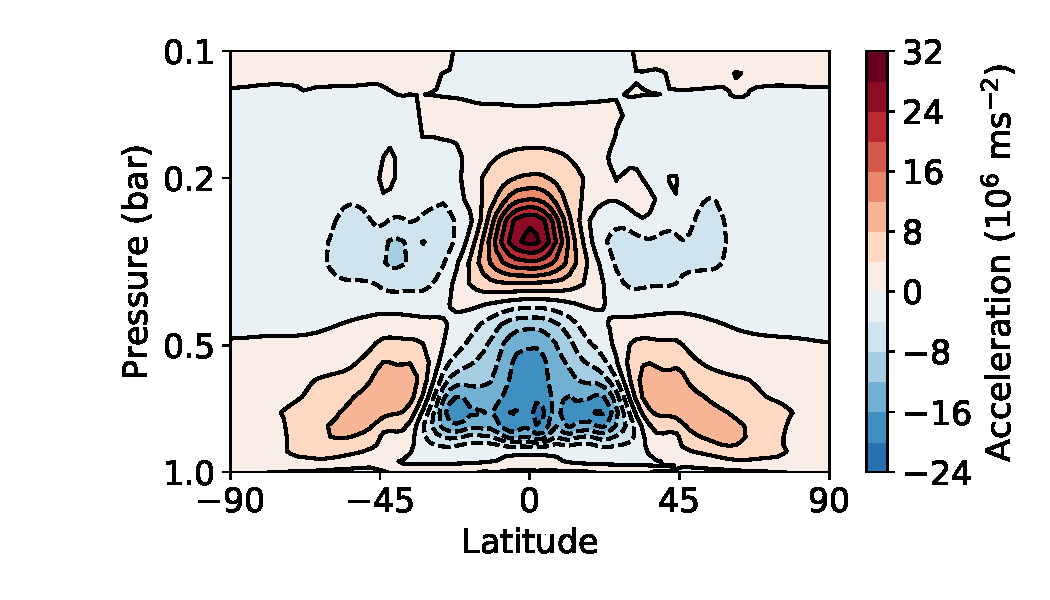
\includegraphics[width=\textwidth]{figures/eqm-zonal-flow/1_flux.pdf}
    \caption{Term Ib, Mean Vertical.}\label{fig:mean-vert}
  \end{subfigure}
  \\
  \begin{subfigure}[t]{0.48\textwidth}
    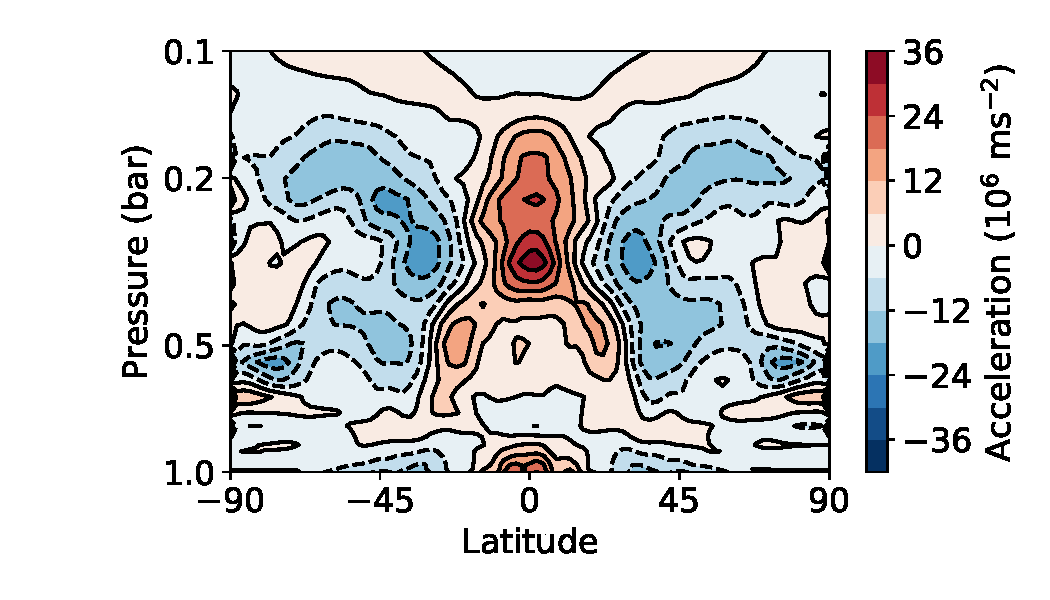
\includegraphics[width=\textwidth]{figures/eqm-zonal-flow/2_flux.pdf}
    \caption{Term IIa, Eddy Horizontal.}\label{fig:stat-horiz}
  \end{subfigure}
\quad
  \begin{subfigure}[t]{0.48\textwidth}
    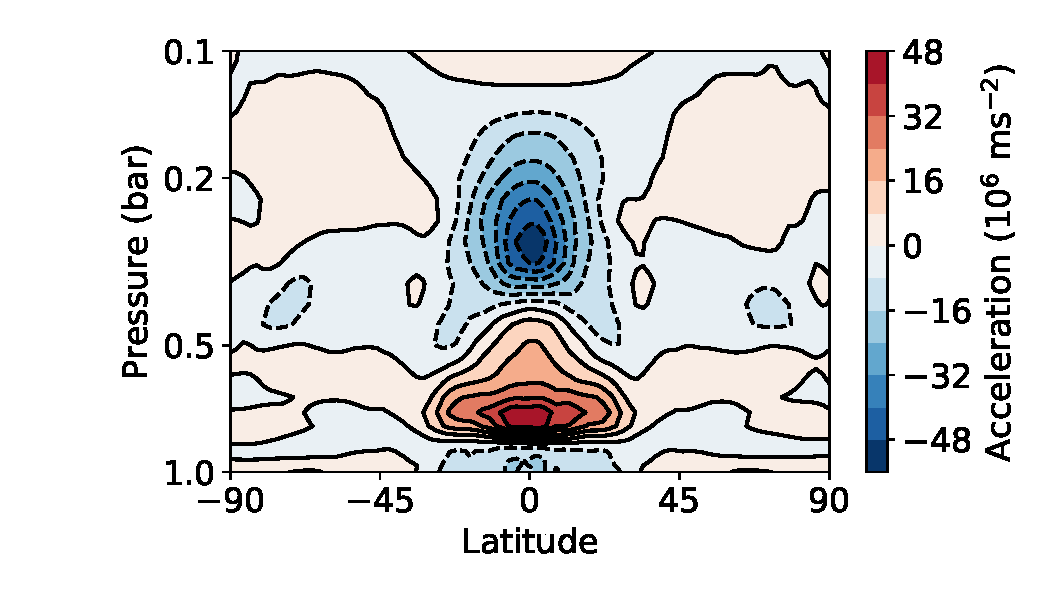
\includegraphics[width=\textwidth]{figures/eqm-zonal-flow/3_flux.pdf}
    \caption{Term IIb, Eddy Vertical.}\label{fig:stat-vert}
  \end{subfigure}
  \caption{The sources of zonal acceleration in Equation \ref{eqn:zonal-mean-mom-gcm}, showing how different terms accelerate and decelerate zonal flow at the equator and at high latitudes. Figure \ref{fig:accn-terms-jet-level} plots these terms at \SI{0.3}{\bar}. }\label{fig:default-gcm-accelerations}
\end{figure}


The ``Mean Vertical'' acceleration of Term Ib is also different to the shallow-water models. It contributes to the eastward acceleration at the equator, opposing Term IIb. This appears to be different to the fluxes in the shallow-water models, where the mean vertical acceleration has no effect. However, Figure \ref{fig:mean-vert} showed that the mean vertical acceleration has a negligible net effect on the strength of the jet, with an acceleration above its centre but a deceleration below its centre. This means that it has no net effect on the strength of the jet, so does not need to be considered when comparing to the single-layer shallow-water models. The balance of acceleration terms in Figure \ref{fig:accn-terms-jet-level} for the GCM is therefore qualitatively the same as the balance of terms in Figure \ref{fig:test-C-accn} for the non-linear shallow-water model, matching the GRW mechanism.

%
% Comparing this to Figure \ref{fig:test-3-accn} shows that the same balance applies in Test C in the non-linear shallow-water model as in Test 1 in the GCM. I suggest that this agreement between the non-linear shallow-water model and the GCM shows that the shallow-water model captures the mechanism forming the zonal flow profile in the GCM. This shows that the important processes in the atmosphere can be split up into the wave-1 day-night forcing, and the wave-0 zonal-mean forcing due to the asymmetry between the day-side cooling and uniform night-side cooling. In the next section, I will use a non-linear shallow-water model to reproduce this process, and show that the same balance of acceleration terms applies.



% \begin{figure}
%   \centering
%   \begin{subfigure}[t]{0.48\textwidth}
%     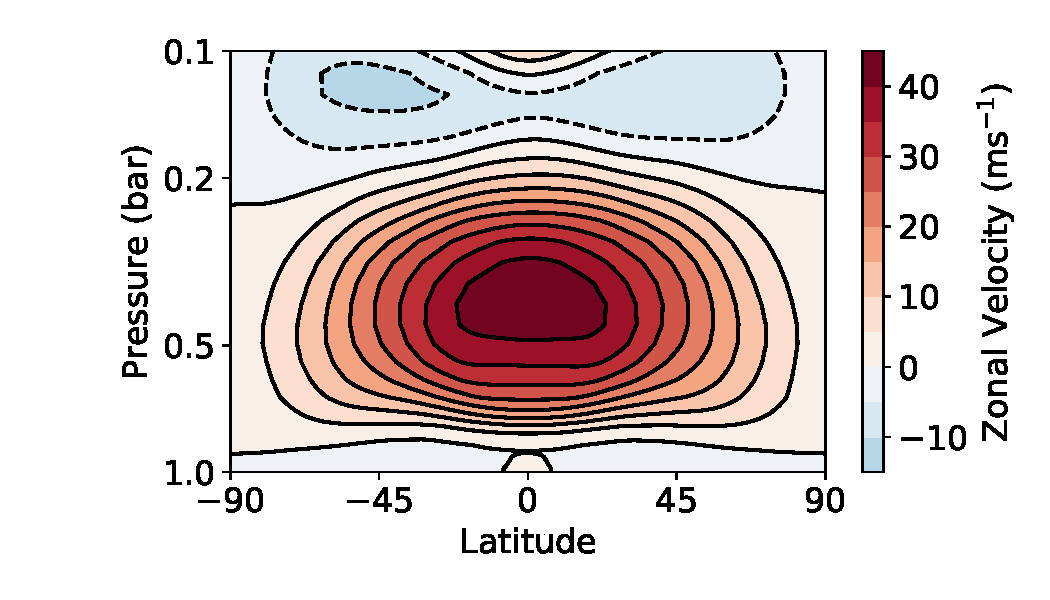
\includegraphics[width=\textwidth]{figures/eqm-zonal-flow/5_flux.pdf}
%     \caption{Zonal-mean zonal velocity.}
%   \end{subfigure}
% \quad
%   \begin{subfigure}[t]{0.48\textwidth}
%     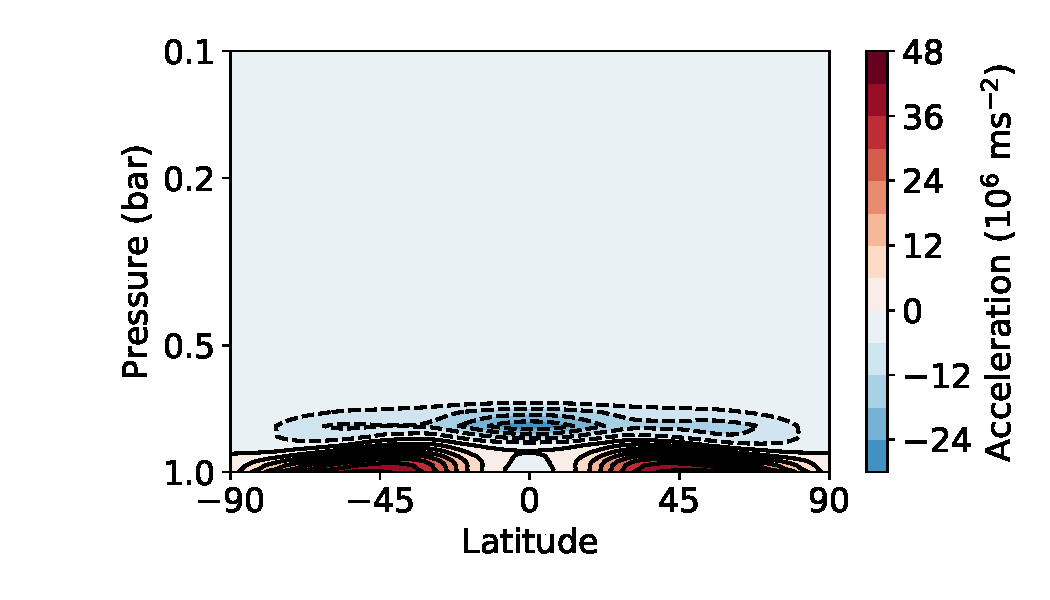
\includegraphics[width=\textwidth]{figures/eqm-zonal-flow/4_flux.pdf}
%     \caption{Acceleration due to Rayleigh drag.}
%   \end{subfigure}
%   \caption{Zonal velocity and drag}
%   \label{fig:default-gcm-velocity-drag}
% \end{figure}



\begin{figure}
  \centering
  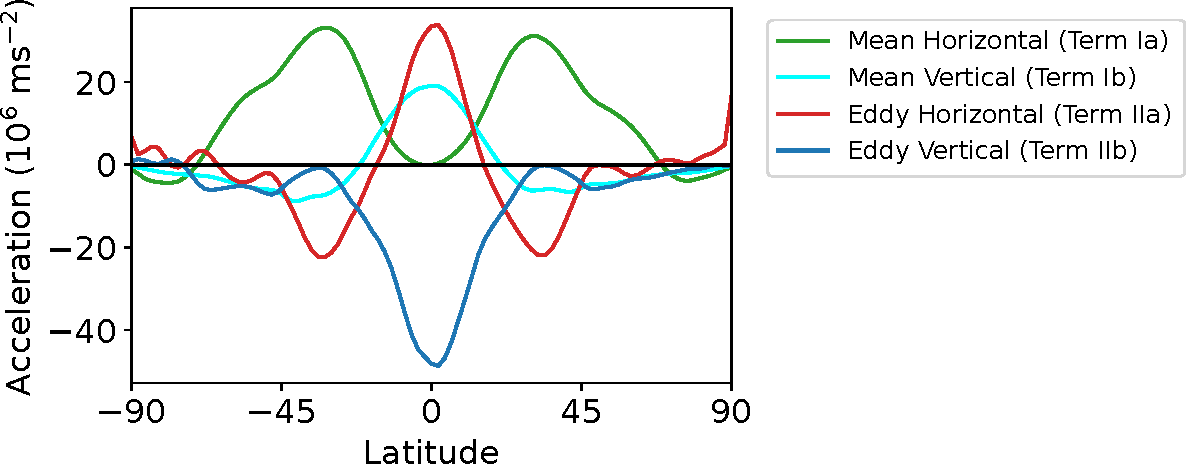
\includegraphics[width=0.9\textwidth]{figures/eqm-zonal-flow/accn-terms-jet-level.pdf}
  \caption{Acceleration terms in the zonal-mean zonal momentum equation at \SI{0.3}{\bar} in Test 1 in Exo-FMS, showing how Terms Ia and IIa in Equation \ref{eqn:zonal-mean-mom-gcm} balance at high latitudes, and that Term IIb balances Terms IIa and Ib at the equator. This matches the shallow-water models in Figures \ref{fig:beta-fluxes-plus-merid} and \ref{fig:test-C-accn}, except for the presence of Term Ib, which is explained in the text.}\label{fig:accn-terms-jet-level}
\end{figure}


%SECTION CONCLUSIONS



%%%%%%%%%%%%%%%%%%%%%%%%%%%%
%SECTION 4 -- SCALING REGIMES
\section{Scaling Behaviour of Zonal Jets on Tidally Locked Planets}

In this section, I will use the ideas developed so far to predict how the strengths and positions of the zonal jets in the atmospheres of tidally locked planets could scale with planetary parameters. \citet{perez2013atmospheric} use a similar non-linear model to derive scaling relations for the global height field and associated day-night contrast. This section will focus on the scaling behaviour of the strength and position of the jets formed on tidally locked planets.


%SUBSECTION -- NONLINEAR MODEL
\subsection{Non-Linear Model Scaling Relations}\label{sec:nonline-scaling-relations}

Equation \ref{eqn:zonal-mean-mom-sphere} shows how each source of acceleration scales with the planetary parameters. Term II drives the equatorial jet, suggesting that the jet speed should scale like $\frac{1}{\overline{h}} \frac{\partial}{\partial y}\left[\overline{(h v)^{\prime} u^{\prime}}\right] \sim u^{\prime} v^{\prime} \sim Q^{2}\alpha^{2}$. Term I in Equation \ref{eqn:zonal-mean-mom-sphere} drives the subtropical jets, suggesting that they should scale like $\overline{v}^{\star}\left[f-\frac{\partial \overline{u}}{\partial y}\right] \sim v^{\prime} f \sim Q\alpha f$.

Figure \ref{fig:u_Q_scaling} shows the scaling of the zonal-mean equatorial and subtropical jet speeds with the forcing strength $\delta h$. Each test has the same parameters as Test C in Section \ref{sec:nonlin-shallow}, except for the magnitude of the forcing. The figure shows that for low forcing values, the equatorial jet does scale quadratically with the forcing (as identified by \citet{showman2011superrotation}), and the subtropical jets scale linearly. For forcing values higher than $\Delta h / h_{0} = 0.01$, the jets increases more slowly than linearity, as non-linear effect become more important. For realistic forcing values of order 0.01 \citep{showman2011superrotation}, the jets still obey this linear scaling trend.

% This test shows that the accelerations of the jets scale as expected in the linear limit, and that the magnitude of forcing required for an approximately linear response is still consistent with that in \citet{showman2011superrotation}.

This predicts that increasing the forcing (instellation) on a tidally locked planet will increase both the equatorial and subtropical jet speeds, and will increase the equatorial jet speed relative to the subtropical jets. In addition, the equatorial acceleration comes at the expense of the subtropical jets due to the equatorward momentum transport, so for very strong forcing the subtropical jets may be replaced by easterly flow.

% Figure \ref{fig:u_Q_scaling} shows the scaling of the zonal-mean equatorial and subtropical jet speeds with damping $\alpha$. Equation \ref{eqn:zonal-mean-mom-sphere} suggests that the equatorial jet should scale quadratically with $\alpha$, and that the subtropical jets should scale linearly. As with the forcing, these behaviour holds up to a value X where the jets increase more slowly with the damping rate. Still realistic X.

% In the next section, I will consider similar scaling relations in the GCM.


\begin{figure}
  \centering
    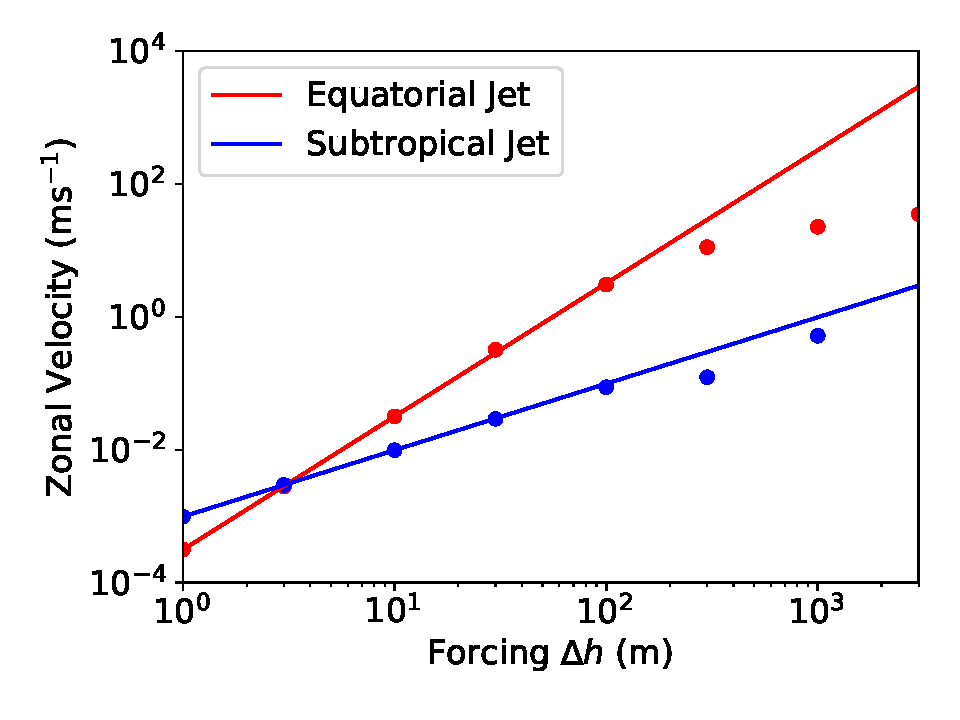
\includegraphics[width=0.8\textwidth]{figures/eqm-zonal-flow/u_Q_scaling.pdf}
  \caption{The equatorial and subtropical jet speeds in the non-linear shallow-water model, versus the magnitude $Q = \delta h /h_{0}$ of the realistic forcing field in Test C, where $h_{0} =$ \SI{1e4}{\metre}. The lines show fits of the predicted quadratic scaling of the equatorial jet, and linear scaling of the subtropic jets.}
  \label{fig:u_Q_scaling}
\end{figure}

% \begin{figure}
%   \centering
%   \begin{subfigure}[t]{0.49\textwidth}
%     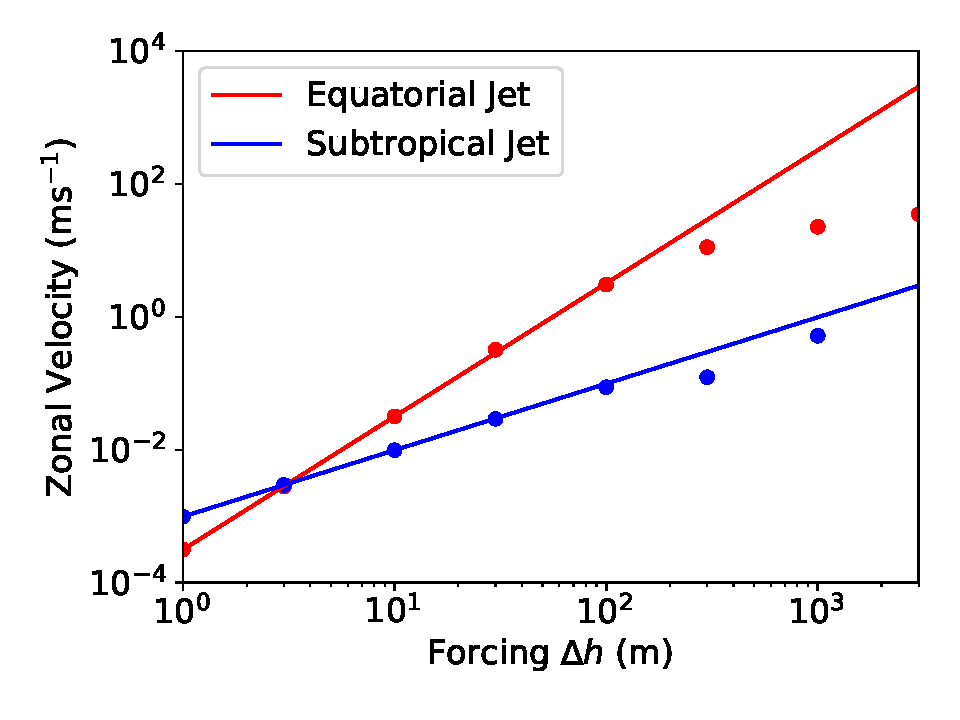
\includegraphics[width=1.0\textwidth]{figures/eqm-zonal-flow/u_Q_scaling.pdf}
%     \caption{Effect of forcing magnitude $Q$.}
%     \label{fig:u_Q_scaling}
%   \end{subfigure}
%   %
%   \begin{subfigure}[t]{0.49\textwidth}
%     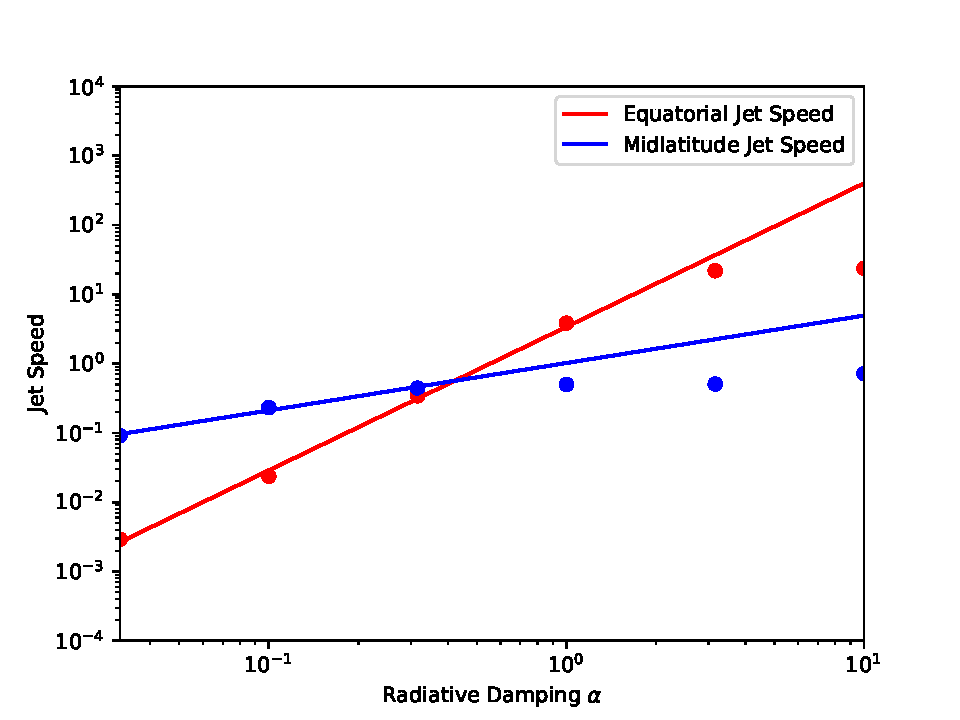
\includegraphics[width=1.0\textwidth]{figures/eqm-zonal-flow/u_alpha_scaling.pdf}
%     \caption{Effect of radiative damping $\alpha$.}
%     \label{fig:u_alpha_scaling}
%   \end{subfigure}
%   \caption{The scaling of the equatorial and subtropical jet speeds in the non-linear shallow-water model, for cases with realistic forcing with variable values of forcing magnitude $Q$ and radiative damping $\alpha$.}
%   \label{fig:nonlin-scaling}
% \end{figure}


%SUBSECTION -- GCM
\subsection{Qualitative GCM Scaling Relations}\label{fig:gcm-qual-scaling}

This section will qualitatively apply the scaling relations from the non-linear shallow-water model to a suite of GCM simulations. Figure \ref{fig:gcm-suite-jets} shows the zonal-mean zonal velocity of nine GCM simulations with different rotation rates and instellation values, adapted from \citet{pierrehumbert2018review}. These tests have a range of zonal flow patterns, with one, two, or three jets of varying strengths and positions, which can be explained with the scaling relations of the previous section.

 Increasing the instellation in the GCM increases the forcing $Q$, and raises the damping rate $\alpha$ due to the higher temperature. I showed previously that increasing the forcing $Q$ and damping $\alpha$ in the shallow-water model increases the strength of all the zonal jets, and increases the strength of the equatorial jet relative to the subtropical jets. This explains why the GCM tests with higher instellation have strong, single equatorial jets, with all the ``hot'' tests having one single jet centred on the equator. The ``hot, 2 day'' test has easterly flow at high latitudes, as the high forcing increases the prograde momentum transport towards the equator.

The GRW mechanism predicts that increasing the rotation rate of the planet should strengthen the subtropical jets, and move them to lower latitudes. This is confirmed by the GCM tests, and is shown most clearly by the ``cold'' cases, where increasing the rotation rate gives faster jets than are closer together. In the ``hot'' simulations, the subtropical jets merge with the equatorial jet and there appears to only be one jet. The GRW mechanism therefore explains the qualitative behaviour of this suite of simulations, and provides an understanding of why GCM simulations of the atmospheres of tidally locked terrestrial planets can have one, two, or three zonal jets of varying strengths.


\begin{figure}
  \centering
  \begin{subfigure}[b]{0.32\textwidth}
    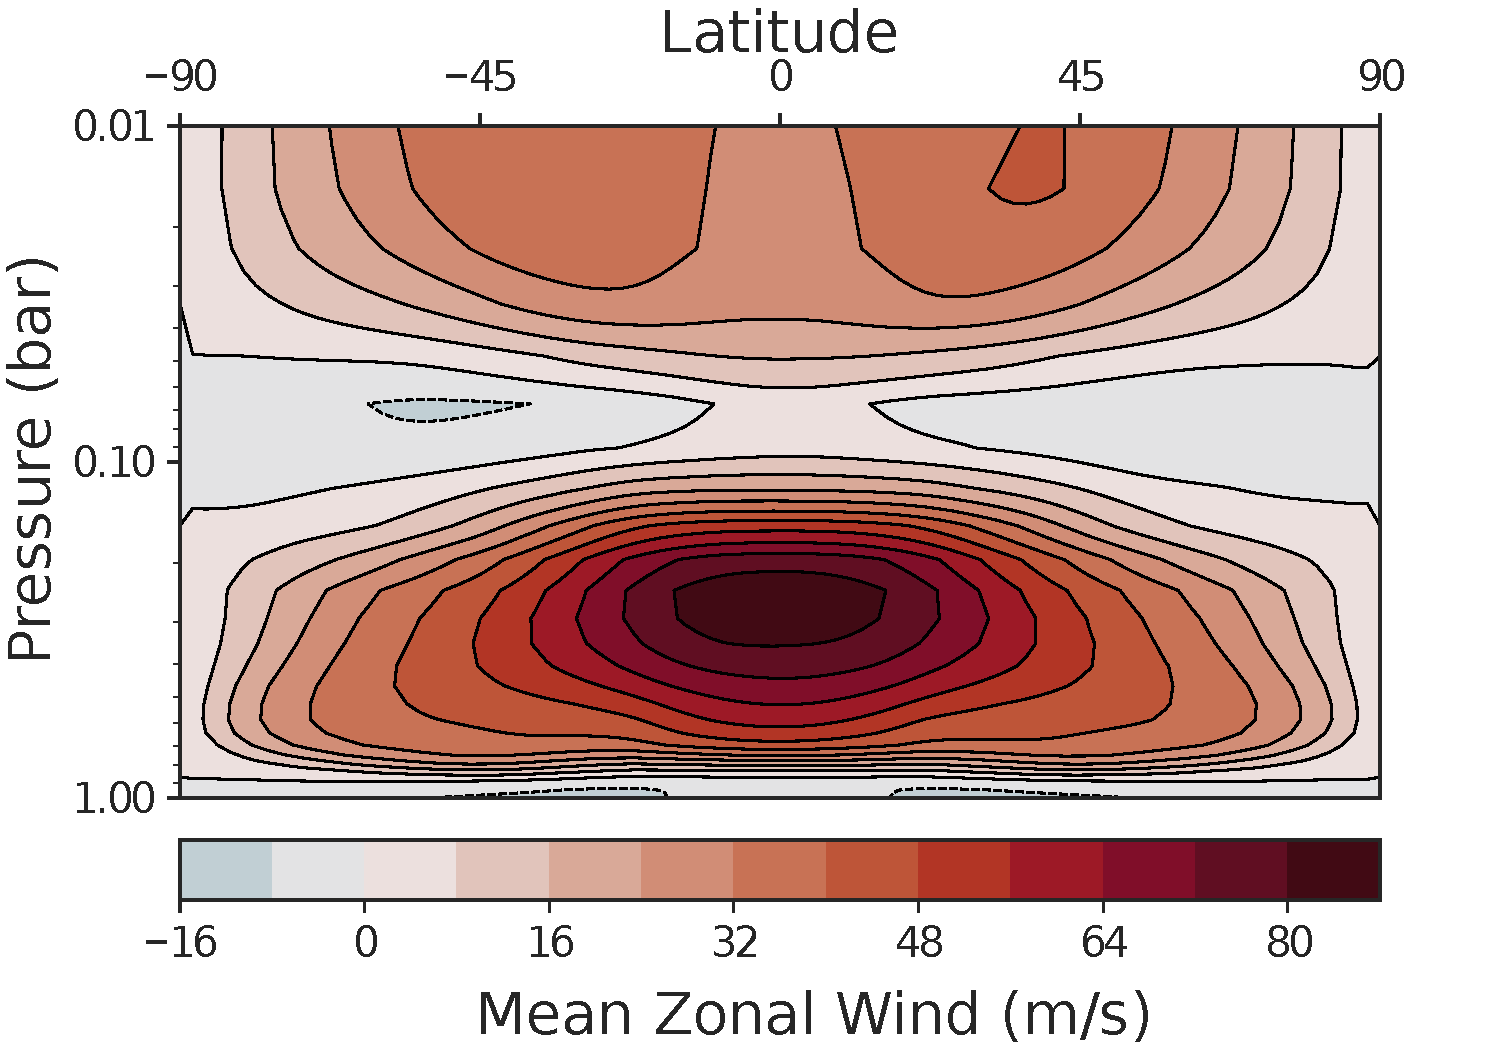
\includegraphics[width=\textwidth]{figures/eqm-zonal-flow/wind-hot-10.pdf}
    \caption{Hot, 10 days.}
  \end{subfigure}
  \begin{subfigure}[b]{0.32\textwidth}
    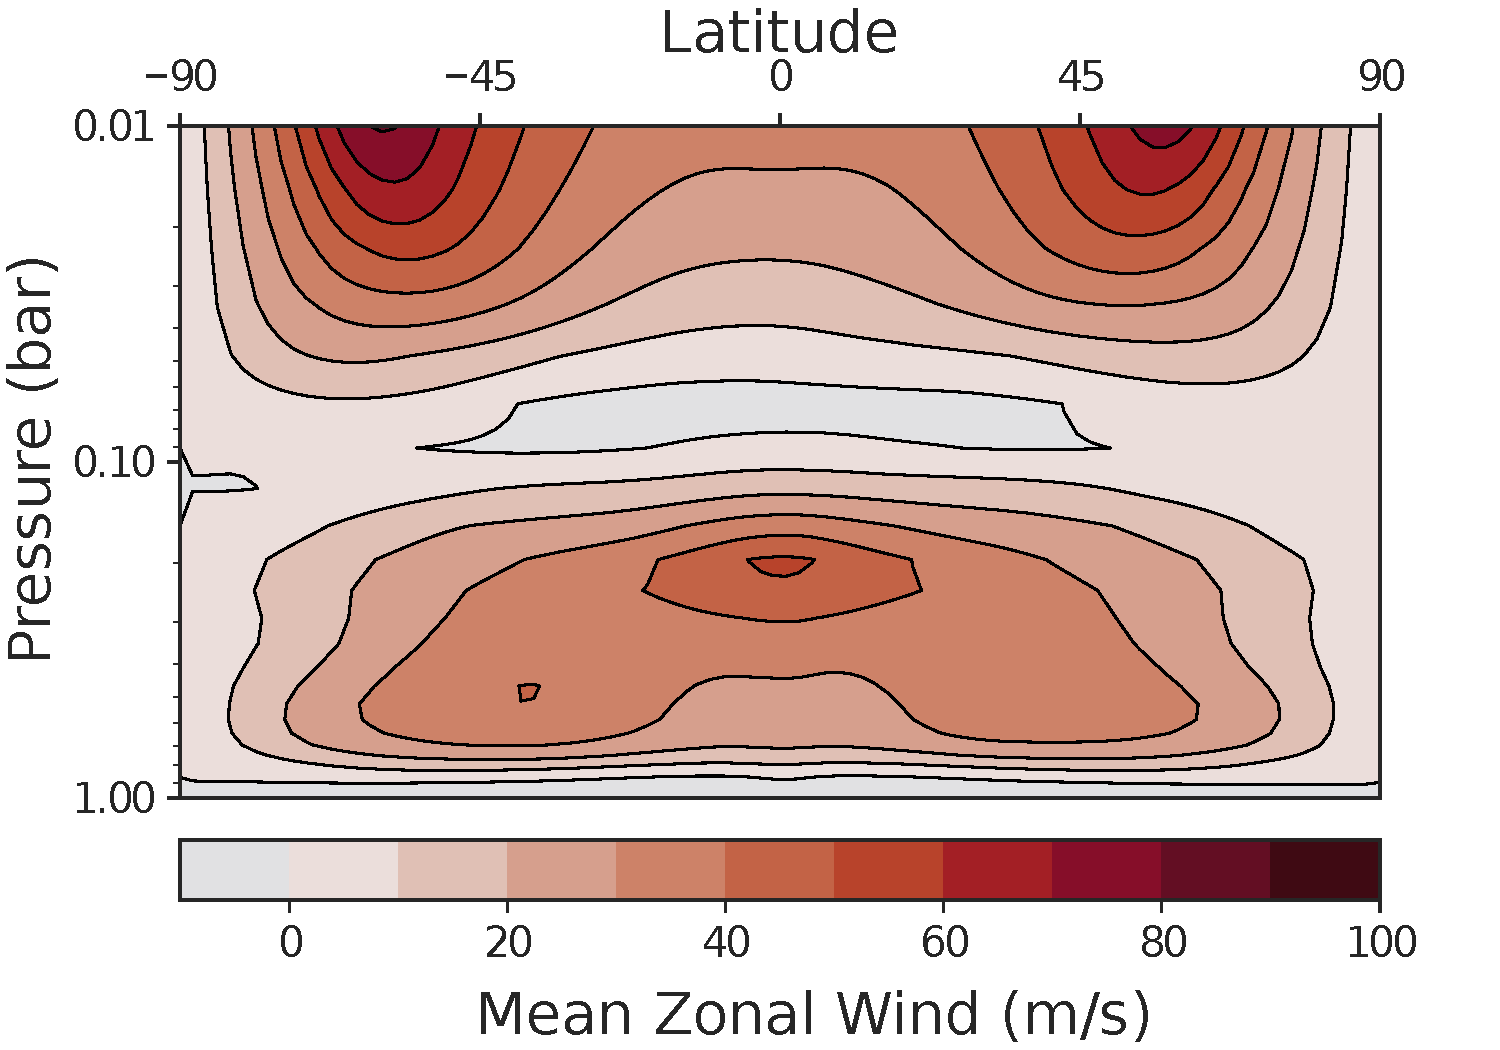
\includegraphics[width=\textwidth]{figures/eqm-zonal-flow/wind-med-10.pdf}
    \caption{Medium, 10 days.}
  \end{subfigure}
  \begin{subfigure}[b]{0.32\textwidth}
    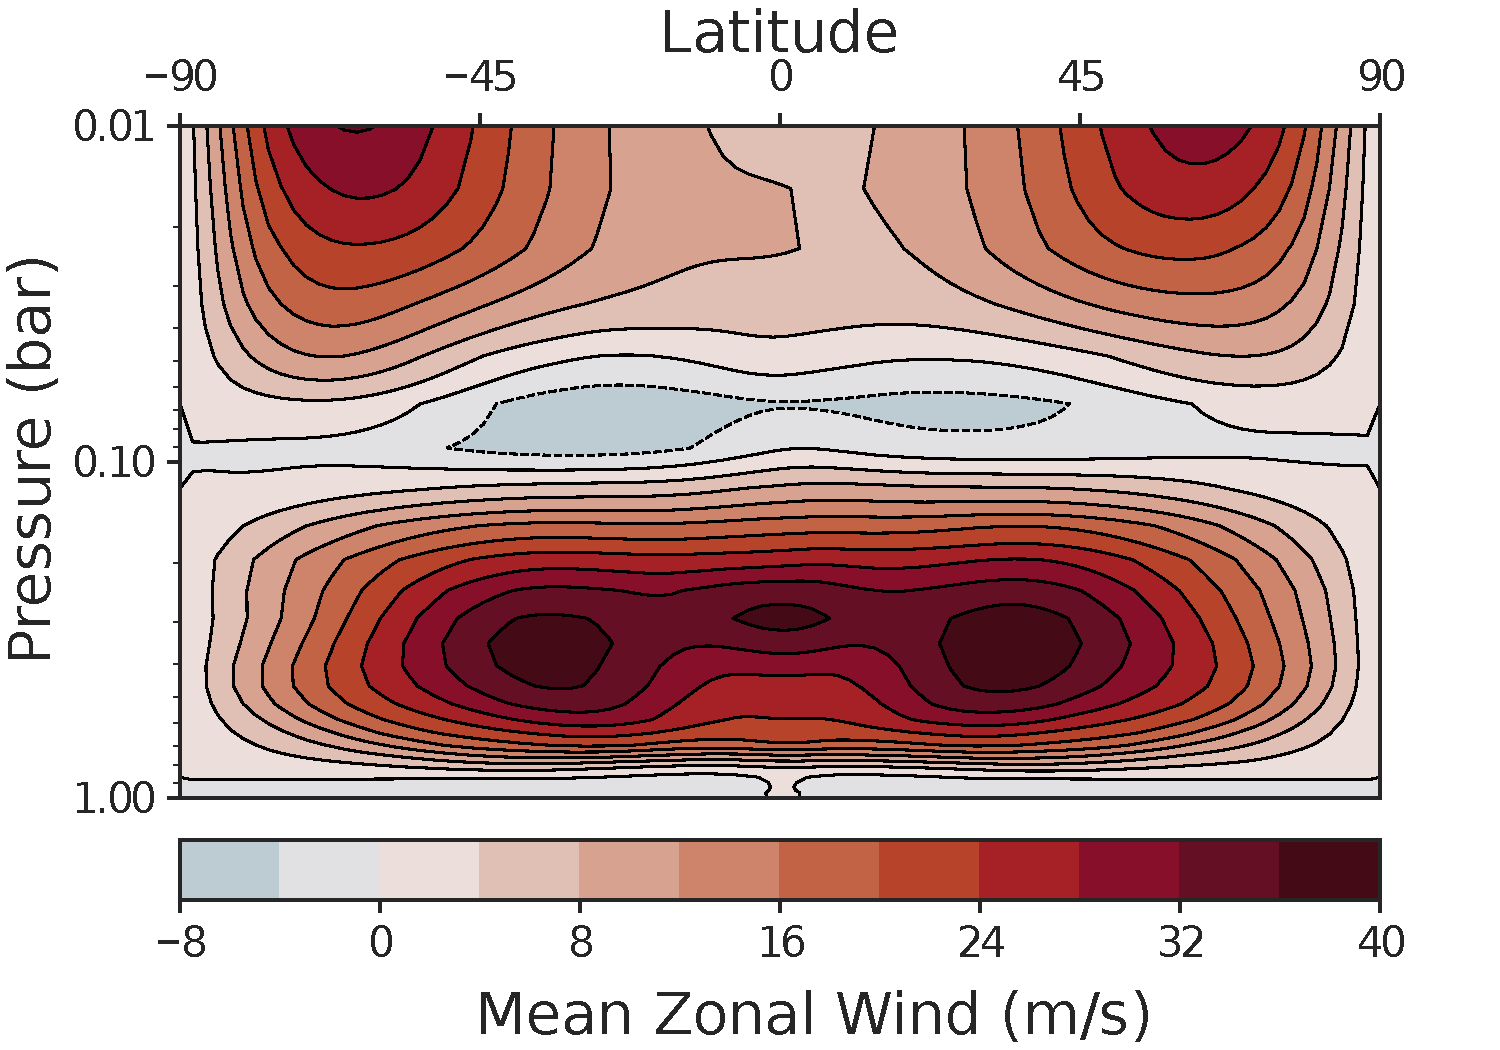
\includegraphics[width=\textwidth]{figures/eqm-zonal-flow/wind-cold-10.pdf}
    \caption{Cold, 10 days.}
  \end{subfigure}
    \\
    \begin{subfigure}[b]{0.32\textwidth}
      \includegraphics[width=\textwidth]{figures/eqm-zonal-flow/wind-hot-5.pdf}
      \caption{Hot, 5 days.}
    \end{subfigure}
    \begin{subfigure}[b]{0.32\textwidth}
      \includegraphics[width=\textwidth]{figures/eqm-zonal-flow/wind-med-5.pdf}
      \caption{Medium, 5 days.}
    \end{subfigure}
    \begin{subfigure}[b]{0.32\textwidth}
      \includegraphics[width=\textwidth]{figures/eqm-zonal-flow/wind-cold-5.pdf}
      \caption{Cold, 5 days.}
    \end{subfigure}
     \\
     \begin{subfigure}[b]{0.32\textwidth}
       \includegraphics[width=\textwidth]{figures/eqm-zonal-flow/wind-hot-2.pdf}
       \caption{Hot, 2 days.}
     \end{subfigure}
     \begin{subfigure}[b]{0.32\textwidth}
       \includegraphics[width=\textwidth]{figures/eqm-zonal-flow/wind-med-2.pdf}
       \caption{Medium, 2 days.}
     \end{subfigure}
     \begin{subfigure}[b]{0.32\textwidth}
       \includegraphics[width=\textwidth]{figures/eqm-zonal-flow/wind-cold-2.pdf}
       \caption{Cold, 2 days.}
     \end{subfigure}
  \caption{Time-mean zonal-mean zonal flow of a suite of tests in the GCM Exo-FMS, showing how the equatorial and subtropical jet speeds and positions depend on instellation and rotation rate. Reproduced with data from \citet{pierrehumbert2018review}.}
  \label{fig:gcm-suite-jets}
\end{figure}

% %SUBSECTION -- GCM
% \subsection{GCM Quantitative Scaling Relations}\label{fig:gcm-quant-scaling}
%
% TO DO


%SECTION CONCLUSIONS



%%%%%%%%%%%%%%%%%%%%%%%%%%%%
%DISCUSSION
\section{Discussion}

This section discusses some complicating aspects of applying the GRW mechanism to real tidally locked planets. The GRW mechanism in Figure \ref{fig:gierasch} assumes that the meridional circulation is global, transporting air from the equator to the pole. This is not the case for a rapidly rotating planet like the Earth, which contains multiple cells of meridional circulation. If a tidally locked planet rotated rapidly enough to limit the meridional extent of these cells, the GRW mechanism might only operate below a certain latitude. This may be the case in the more rapidly rotating tests in Figure \ref{fig:gcm-qual-scaling}, where the subtropical jets are closer to the equator and there is easterly flow at high latitudes. However, these tests show that a global meridional circulation is not strictly necessary for the GRW mechanism to function. A limited meridional circulation still receives westerly angular momentum from the surface and conveys it to the jet layer. The subtropical jets will be closer to the equator, and the behaviour at high latitudes may be different.

The meridional circulation is more complicated on tidally locked gas giants like hot Jupiters, which do not have a surface to bound the meridional circulation and apply drag to its lower branch. \citet{heng2011atmospheric} and \citet{mendoncca2018revisiting} showed that the meridional circulation of a hot Jupiter has a direct Hadley-cell like circulation above a certain pressure level, with indirect cells below it, which is similar to some models of Venus \citep{sugimoto2019fully}. The equatorial superrotation in these hot Jupiter simulations is still in the same region as the direct cells, so the GRW mechanism may still describe the formation of the zonal flow. Hot Jupiter simulations still often apply drag to their lower boundary \citep{liu2013atmospheric}, which could add angular momentum to the atmosphere and produce a meridional circulation. The deep atmosphere may fulfil the same role as a surface if there is no explicit bottom drag, providing a reservoir for retrograde flow deep down.
 %
 % It is possible that the transition between the direct and indirect corresponds to the level of heating. The direct cells then behave as in the terrestrial case. In gas giants, they may act the same as the surface in the terrestrial case, linking the upper level flow to the deep atmosphere or an imposed surface. The drag from this surface can then act the same as the drag from a terrestrial surface, although it is applied via the indirect cells.

Finally, this chapter has not considered an important mechanism discussed in detail for hot Jupiters by \citet{showman2015circulation} -- the formation of westerly midlatitude jets by baroclinic instability. This can transport enough westerly momentum away from the equator to reduce the strength of the equatorial jet, and even to reverse its direction. This could be added to the GRW mechanism as another source of horizontal transport of zonal momentum in the layer of the jet. \citet{laraia2015superrotation} considered a similar situation on non-tidally locked planets, estimating the effect of both equatorward momentum transport due to equatorial waves, and transport away from the equator due to baroclinic instability. This additional transport is only important for more rapidly rotating planets, and so is not important for planets such as those simulated earlier with 10 day periods. However, in a full consideration of the formation of zonal flow on tidally locked planets it cannot be ignored, especially for hot Jupiters or more rapidly rotating terrestrial planets. It may be possible to classify planets into different regimes, where either the meridional circulation, stationary wave forcing, or baroclinic instability dominates the formation of zonal jets \citep{showman2015circulation}.

%%%%%%%%%%%%%%%%%%%%%%%%%%%%
% %BALANCE
% \section{Equatorial Momentum Balance}
%
% How does a zonal flow affect the acceleration terms at the equator?
%
% If any deceleration terms monotonically decrease with mean zonal flow, the linear model underpredicts the equilibrium speed.
%
% The two terms that can do this are the drag, and the R. Drag doesn't act on the jet (could it act indirectly, through transport -- it sort of does, via dragging the air transported down by the stationary vertical eddy term).
%
% The other term R depends on total u in SP2011. But, the stationary eddy term in the linear model depends on eddy u. The stationary mean term must be zero in the linear model. So that leaves the mean R term, eddy R term, and the eddy terms in the linear model.
%
% Compare these to the vertical eddy and mean terms in the GCM (which include R). In the GCM, the mean term moves the jet up, with little actual effect on column momentum (as it isn't moving air into a dragged region?). The vertical term provides a large deceleration as it moves air down into a dragged region.
%
% So, for zero mean flow all the acceleration terms are the same.
%
% For mean flow, the eddy terms are the same (modified by resonance and Doppler-shift). All the mean term does is move the jet up, with only a small net deceleration due to delta U of omega column.
%
% So the jet is dragged by the mean vertical delta U, and Rayleigh drag from downward eddy transport into boundary layer.
%
%
% MAIN POINT: vertical mean transport only has effect of delta U between surface (BL) and top of omega column (above jet)? This increases with U, but is only a fraction of it in the shallow-water model. Delta U either due to surface easterlies, or residual westerlies above jet core.
%
% Can we go one step further and suggest that only the subsiding air matters, so only the subsiding part of the vertical eddy term matters in the vertical?

% \section{Effect on hot Jupiters}
%
% Kataria, Drummond get opposite high latitude flow. Possibly caused by surface drag in Kataria (and all MITgcm).
%
% Set up ExoFMS hot Jupiter (WASP19b?). Run with and without drag, compare high latitude jets.


%%%%%%%%%%%%%%%%%%%%%%%%%%%%
%CONCLUSIONS
\section{Conclusions}

This chapter has shown how the Gierasch-Rossow-Williams mechanism describes the formation of the zonal flow at all latitudes in the atmospheres of tidally locked terrestrial planets. I demonstrated this mechanism in a linear shallow-water model, a non-linear shallow-water model, and the GCM Exo-FMS. All these models predicted that equilibrium was produced by the same balance of sources of acceleration in the zonal-mean zonal momentum equations. This mechanism correctly predicted how the zonal flow at the equator and at high latitudes scaled with forcing in the non-linear shallow-water model. It also explained the qualitative scaling behaviour of the strength and position of the zonal jets formed in a suite of idealised GCM simulations.

Further work should consider the role of this mechanism in the formation of zonal flow in the atmospheres of hot Jupiters, which have observable features that depend on their zonal flow \citep{showman2015circulation}. The role of the surface drag in the GRW mechanism suggests that the presence of drag in a hot Jupiter GCM may be vital to the form and strength of its equilibrium zonal flow \citep{cho2015sensitivity}. Understanding the formation process in detail would also help to understand the approximations that are possible in accurate simulations \citep{mayne2019limits}, and to predict the scaling behaviour of observable features such as the jet speed or hot-spot shift \citep{zellem2014hd209, louden2015spatially}.

In conclusion, the GRW mechanism can explain the formation and equilibration of the zonal flow on terrestrial tidally locked planets. It allows for eastward flow at all latitudes, unlike the shallow-water model of \citet{showman2011superrotation} that does not match some GCM simulations. The next chapter will investigate the effect of this zonal flow on the global circulation and observable temperature distribution of the atmospheres of tidally locked planets.

%%%%%



%RESTATE SECTION CONCLUSIONS

%OPEN OUT CONCLUSIONS


% \bibliographystyle{unsrtnat}
% \bibliography{../references.bib}
